%%%%%%%%%%%%%%%%%%%%%%%%%%%%%%%%%%%%%%%%%%%%%%%%%%%%%%%%%%%
\section{Apresentação dos dados}

A base de dados BloodMNIST é formada por um total de 15380 imagens de células sanguíneas divdidas em 8 classes, como mostrado na \autoref{fig:samples_of_classes}. Essas amostras se dividem em conjunto de treinamento, com 11959 representantes e teste, com 3421 itens. As imagens estão disponíveis em diferentes resoluções, sendo \textit{a priori}, escolhida a resolução de 28x28 para trazer uma maior eficiência computacional, principalmente para o caso das redes densas. \textbf{Porém, propõem-se o teste de amostras de maior resolução para a rede convolucional já treinada com as amostras 28x28, para validação da robustez ao tamanho da entrada.}

\begin{figure}[H]
	\centering
	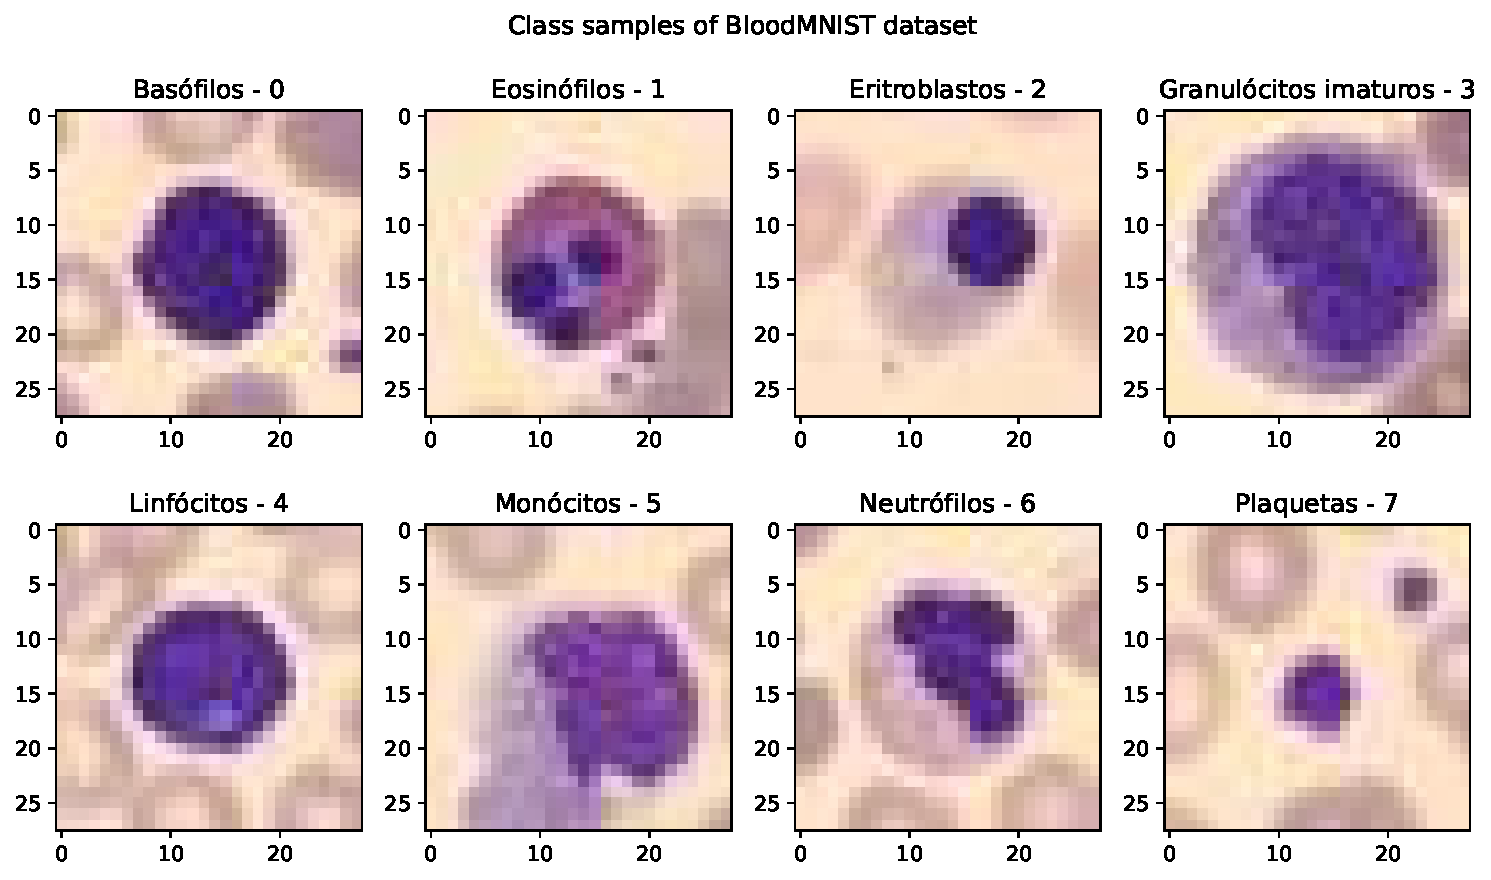
\includegraphics[width=0.75\linewidth]{../../plot/samples_of_classes}
	\caption{Amostras das classes do \textit{dataset} BloodMNIST.}
	\label{fig:samples_of_classes}
\end{figure}

O \textit{dataset} BloodMNIST já fornece de forma separada os dados utilizados para treinamento, e os que serão utilizados para teste. A \autoref{fig:balancingofclasses} mostra a distribuição de amostrar para cada classe, para os conjuntos de treinamento, em azul, e de teste, em verde. Observa-se que existem classes majoritárias, como a 1, 3, 6 e 7, que apresentam muito mais amostras que as demais. O perfil de amostras por classe é similar nos conjuntos de teste e treinamento, o que mostra que o impacto no mapeamento pelo desbalanceamento das classes irá afetar de forma igual ambos os \textit{datasets}. \textbf{Tal disparidade pode ser tanto causada por um viés na coleta de dados, quanto também pela ocorrência real de mais representantes de uma classe do que das demais, o que modela de forma realista os dados.}

% TODO: \usepackage{graphicx} required
\begin{figure}[H]
	\centering
	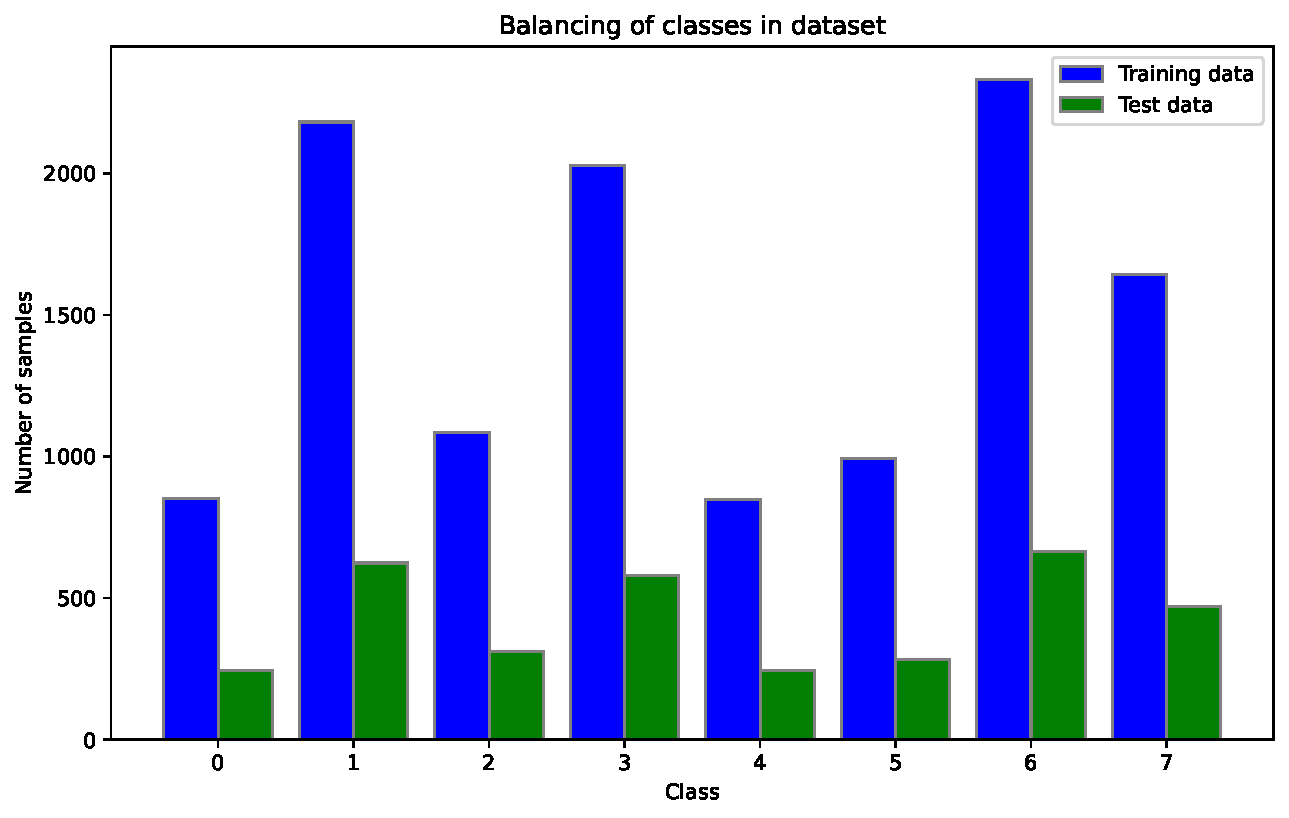
\includegraphics[width=0.75\linewidth]{../../plot/Balancing_of_classes}
	\caption{Balanço das classes nos \textit{datasets} de treinamento e teste.}
	\label{fig:balancingofclasses}
\end{figure}

Para realizar o treinamento utilizando da ferramenta de validação cruzada, foi escolhida a validação do tipo \textit{holdout}, por meio do particionamento do conjunto de dados de treinamento, obtendo um novo conjunto de dados de validação. O novo conjunto de treinamento é formado pelos primeiros 70\% do conjunto original de treinamento, enquanto o de validação, os 30\% restantes do final do \textit{dataset} original. Para garantir a veracidade da validação, quer-se que ambos os conjuntos tenham a mesma representação de cada classe, o que pode se afirmar positivo de acordo com a \autoref{fig:balancingofclasses_holdout}.

% TODO: \usepackage{graphicx} required
\begin{figure}[H]
\centering
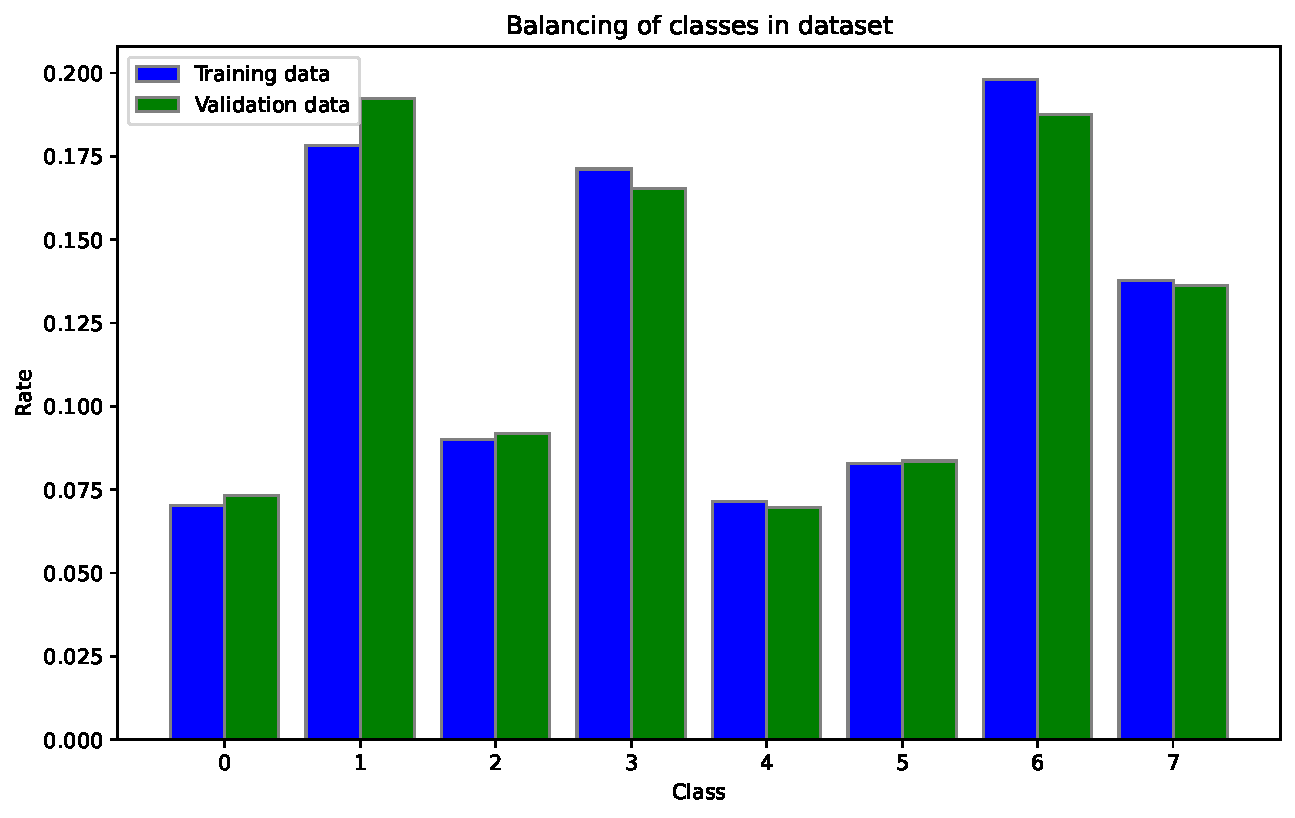
\includegraphics[width=0.75\linewidth]{../../plot/Balancing_of_classes_holdout}
\caption{Balanço das classes nos conjuntos de dados de treinamento e validação cruzada do tipo \textit{holdout}.}
\label{fig:balancingofclasses_holdout}
\end{figure}




%%%%%%%%%%%%%%%%%%%%%%%%%%%%%%%%%%%%%%%%%%%%%%%%%%%%%%%%%%%%%%%%%%%%%%%%%%%%%%%%%%%%%%%%%
\clearpage
\section{MLP}

A implementação da rede MLP com uma camada intermediária se deu por meio do uso do \textit{framework} TensorFlow, possuindo uma camada de entrada que sequencia os pixels da imagem em um vetor, uma camada de neurônios intermediária, e uma camada de saída com função de ativação \textit{softmax} para geração do vetor \textit{one-hot encoding} das probabilidades da entrada pertencer à cada uma das 8 classes.

\subsection{Busca do melhor modelo}

Para realizar a busca do melhor modelo da MLP, considerando que existem uma grande possibilidade de hiper-parâmetros, foi realizada uma busca exaustiva simplificada por etapas, baseada no funcionamento dos \textit{wrappers}, onde dada uma configuração inicial de parâmetros, baseado no comumente visto na literatura \cite{geron2019hands}. As variáveis selecionadas para a busca foram: Número de neurônios da camada intermediária, função de ativação dos neurônios da camada intermediária, taxa de \textit{dropout} dos neurônios da camada intermediária e otimizador para ajuste dos pesos. Demais hiper-parâmetros como tamanho do \textit{batch} e passo do algoritmo de otimização foram mantidos \textit{default}.

A busca por etapas se deu da seguinte forma: Dada a condição inicial, uma MLP de 256 neurônios na camada intermediária com função de ativação ReLU, sem \textit{dropout} e ajustada por \textit{Stochastic Gradient Descendent} (SGD), testou-se a rede alterando primeiramente o número de neurônios. Uma vez conhecido o valor que obteve maior acurácia, testou-se as funções de ativações canditadas para esse número de neurônios, buscando a combinação que desse a melhor acurácia. O processo se repete para o \textit{dropout} e o algoritmo de otimização, onde ao final se obtém a combinação que agrega o melhor número de neurônios visto, melhor função de ativação para tal conjunto de neurônios, melhor taxa de \textit{dropout} e o melhor otimizador.

Hiper-parâmetros variados durante a busca:


\begin{itemize}
	\item Número de neurônios: [ \texttt{256}; \texttt{512}; \texttt{1024}; \texttt{2048}; \texttt{4096} ]
	\item Função de ativação: [ \texttt{ReLU}; \texttt{Sigmoide} ]
	\item \textit{Dropout}: [ \texttt{0,0}; \texttt{0,25}; \texttt{0,5} ]
	\item Otimizador: [ \texttt{SGD}; \texttt{ADAM} ]
\end{itemize} 

Para todos os casos, foram treinadas 500 épocas, com \textit{mini-batch} de 32 amostras, utilizando uma função de \textit{callback} para salvar os parâmetros da melhor época, evitando assim preocupações com \textit{overfitting}.

\subsubsection{Número de neurônios}

Com intuito de definir a quantidade de neurônios que irão compor a camada intermediária da MLP, treinou-se a rede para camadas intermediárias com 256, 512, 1024, 2048 e 4096 neurônios, monitorando a perda e a acurácia para os dados de treinamento e de validação. Os gráficos da \autoref{fig:search_neurons_training}, mostram a evolução dessas medidas ao longo das épocas. Observa-se que para todos os casos, ocorre \textit{overfitting} no treinamento, onde a perda de validação, em vermelho, começa a apresentar uma elevação na sua curva ruidosa. Porém, como o treinamento foi realizado salvando o conjunto de pesos da melhor época, não se faz um problema treinar o modelo mais épocas do que o necessário.



Ao analisar a acurácia e perda de validação para cada um dos modelos treinados com uma quantidade diferente de neurônios na camada intermediária, obtém-se a \autoref{fig:search_neurons}. Como esperado, ao aumentar o número de neurônios se aumenta a acurácia e reduz a perda, uma vez que a rede se torna mais flexível e consegue aproximar mais o mapeamento alvo do treinamento. Porém, com o aumento da flexibilidade da máquina, o treinamento também se torna mais desafiador, sendo necessários uma grande quantidade de dados para maximizar a generalização do modelo.

Considerando todos os números de neurônios utilizados, não há um aumento estrondoso da acurácia, mostrando que para todos eles, o mapeamento pode ser bem aproximado, porém, a redução da perda é considerável considerando a rede com camada intermediária de 256 neurônios e a de 4096 neurônios. Observando a forma da curva de acuária, é perceptível que a taxa de crescimento apresenta uma saturação, ou seja, o valor máximo da acurácia que pode ser atingido por essa arquitetura de rede neural tende a atingir um valor máximo.

Com isso, a camada intermediária de 4096 neurônios foi escolhida para a rede final, e será utilizada nas buscas dos hiper-parâmetros subsequentes.




\begin{figure}[H]
	\centering
	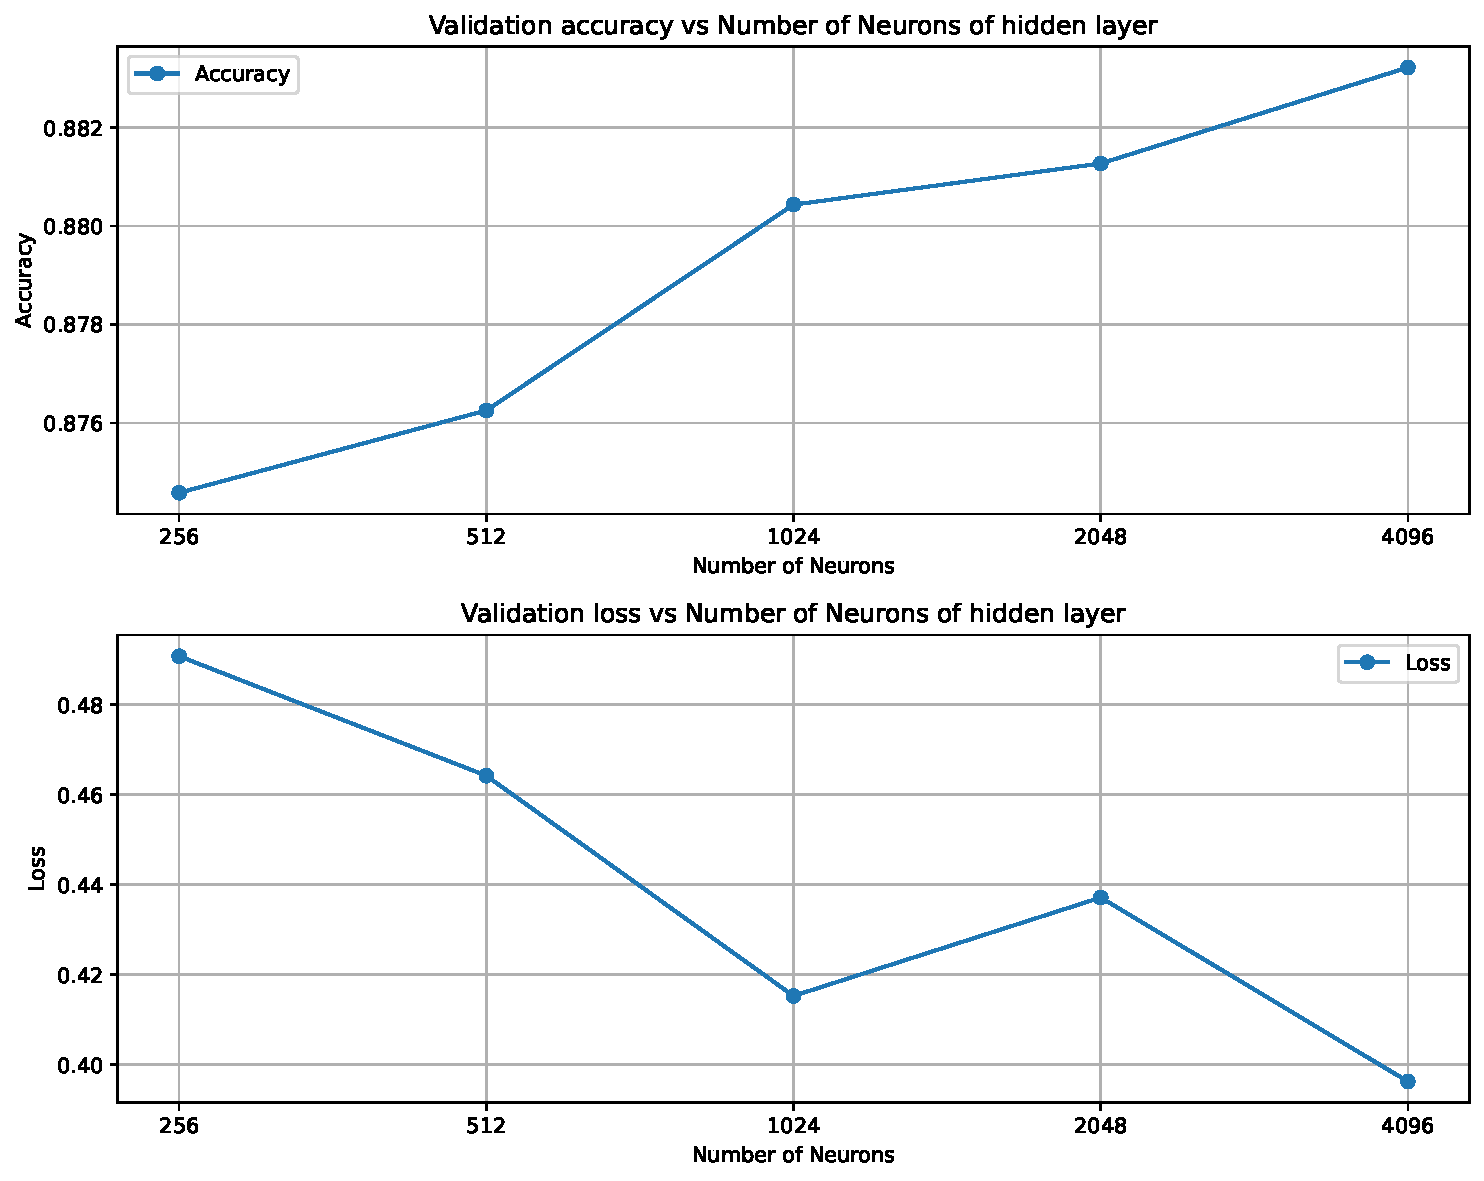
\includegraphics[width=0.75\linewidth]{../../plot/mlp/search_neurons}
	\caption{Acurácia e perda com a variação do número de neurônios da camada intermediária.}
	\label{fig:search_neurons}
\end{figure}

\begin{figure}[H]
	\centering
	\begin{subfigure}[H]{0.49\textwidth}
		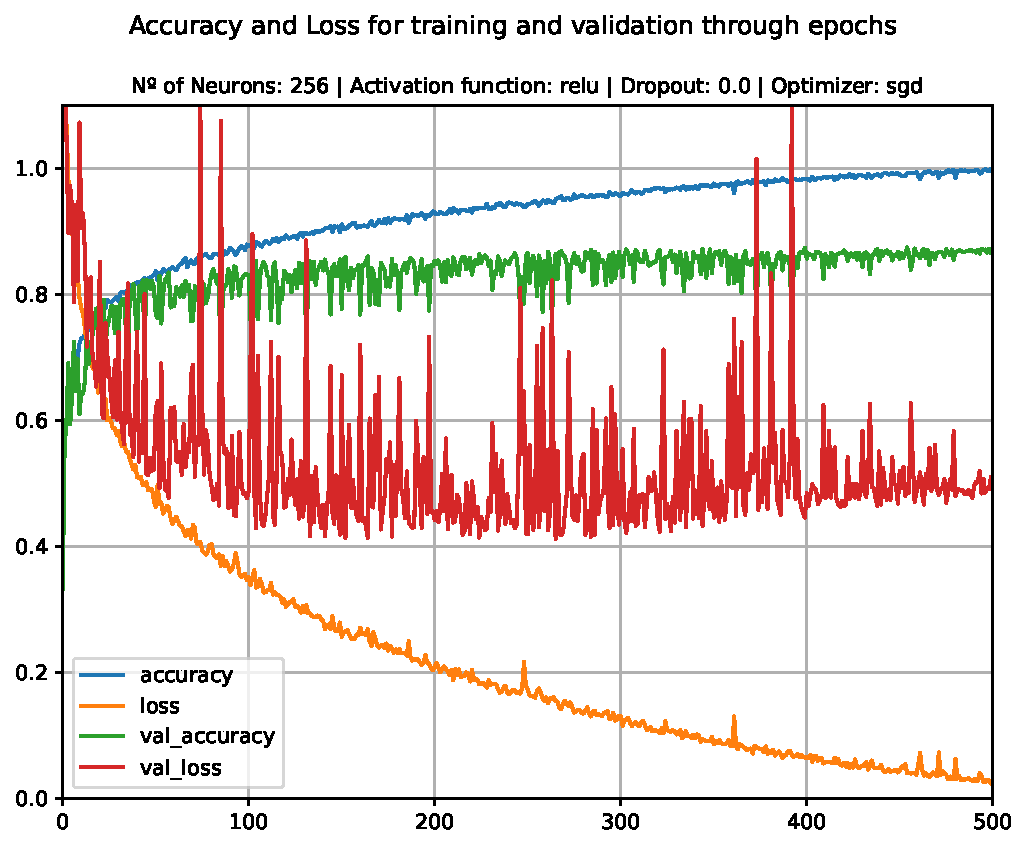
\includegraphics[width = \textwidth]{../../plot/mlp/mlp_256_relu_0.0_sgd}
		\caption{256 neurônios.}
		\label{fig:mlp_256_relu_0.0_sgd}
	\end{subfigure}
	\begin{subfigure}[H]{0.49\textwidth}
		\centering
		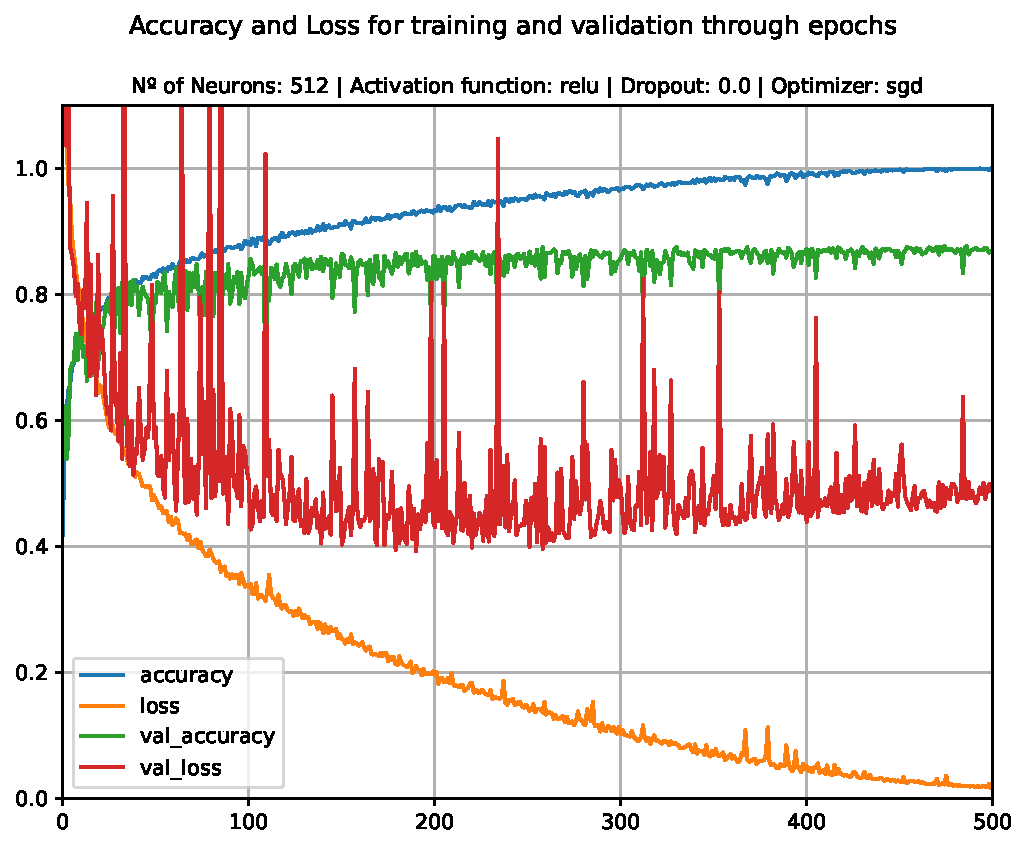
\includegraphics[width = \textwidth]{../../plot/mlp/mlp_512_relu_0.0_sgd}
		\caption{512 neurônios.}
		\label{fig:mlp_512_relu_0.0_sgd}
	\end{subfigure}
	\begin{subfigure}[H]{0.49\textwidth}
		\centering
		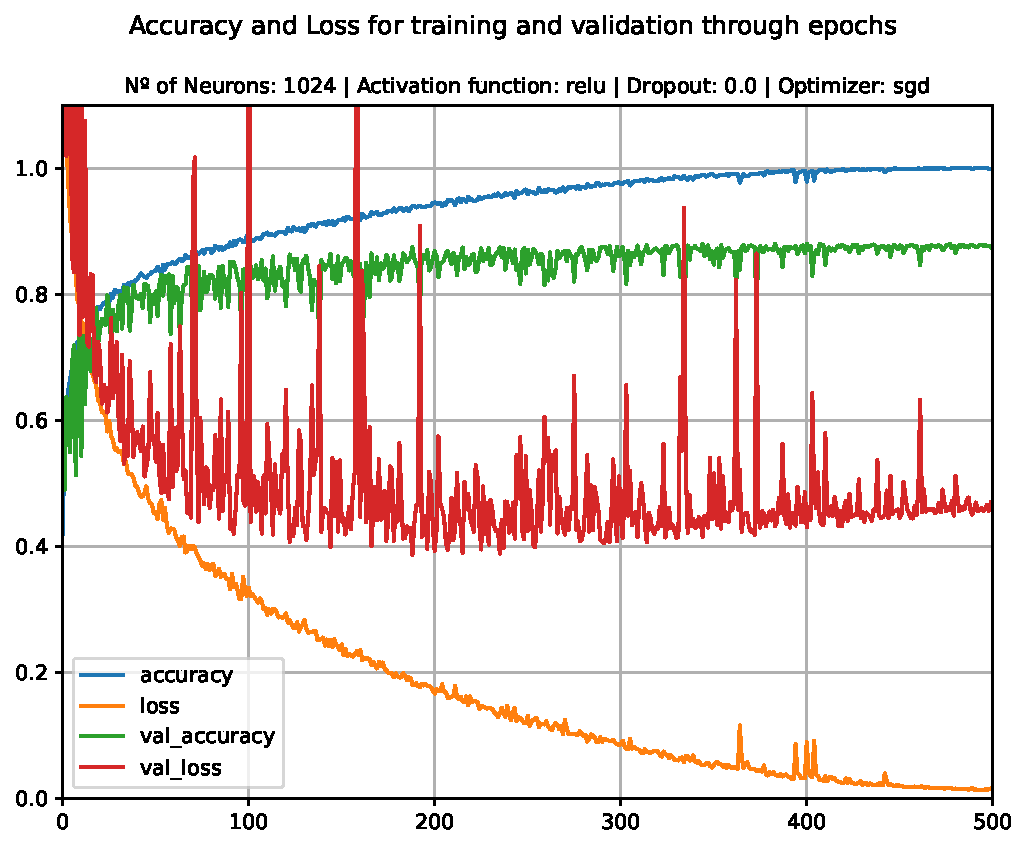
\includegraphics[width = \textwidth]{../../plot/mlp/mlp_1024_relu_0.0_sgd}
		\caption{1024 neurônios.}
		\label{fig:mlp_1024_relu_0.0_sgd}
	\end{subfigure}
	\begin{subfigure}[H]{0.49\textwidth}
		\centering
		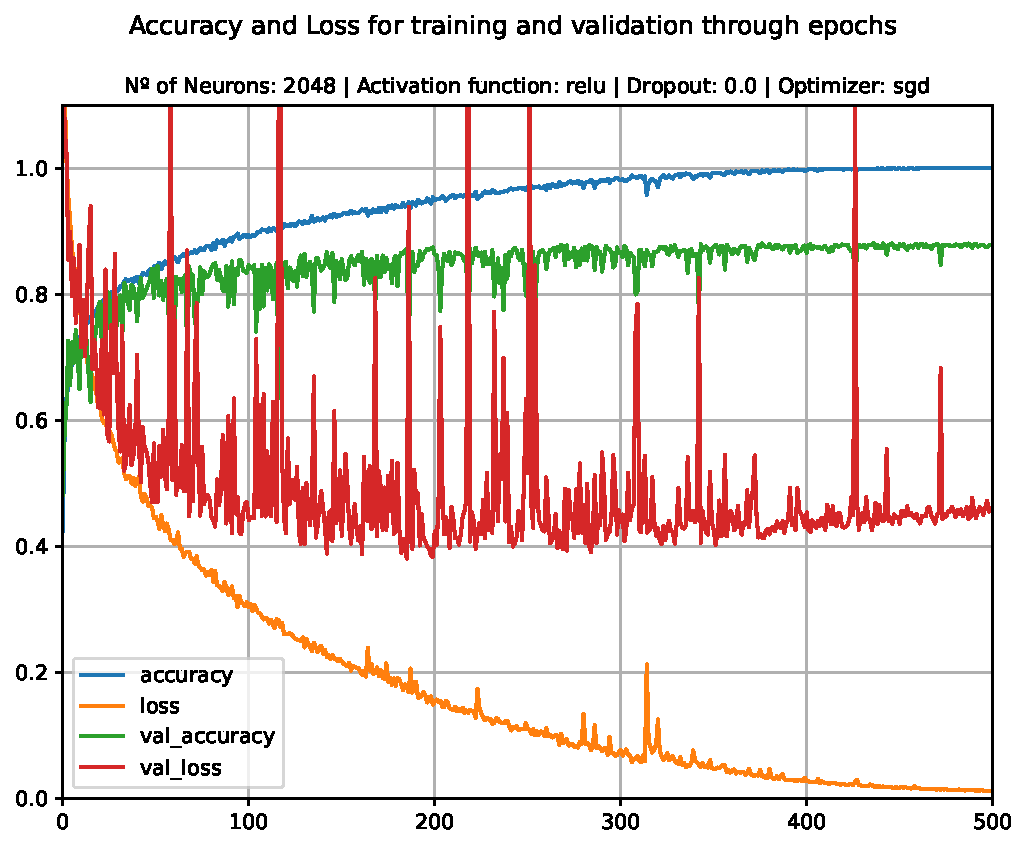
\includegraphics[width = \textwidth]{../../plot/mlp/mlp_2048_relu_0.0_sgd}
		\caption{2048 neurônios.}
		\label{fig:mlp_2048_relu_0.0_sgd}
	\end{subfigure}
	\begin{subfigure}[H]{0.49\textwidth}
		\centering
		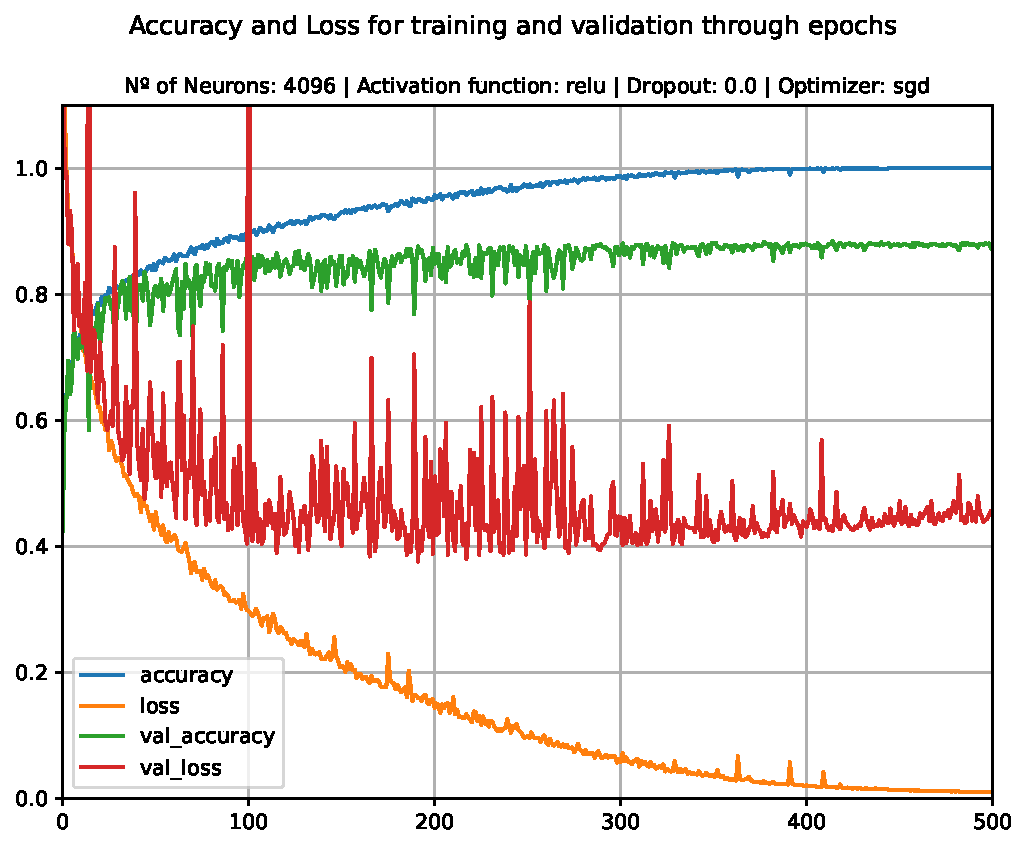
\includegraphics[width = \textwidth]{../../plot/mlp/mlp_4096_relu_0.0_sgd}
		\caption{4096 neurônios.}
		\label{fig:mlp_4096_relu_0.0_sgd}
	\end{subfigure}
	\caption{Evolução da perda e acurácia de treinamento e validação com as épocas de treinamento para cada número de neurônios avaliados.}
	\label{fig:search_neurons_training}
\end{figure}

\subsubsection{Função de ativação}

	A função de ativação é a responsável por dar um mapeamento não-linear para a MLP, dessa forma, sua escolha é crucial para viabilizar o treinamento da rede, assim como para garantir a capacidade de generalização da mesma. Foram escolhidas duas funções de ativação com características diferentes, a ReLU, que executa a operação de um retificador linear, e a sigmoide, que varia seu valor de 0 a 1 na forma de uma função logística. 
	
	A \autoref{fig:mlp_4096_relu_0.0_sgd_act_fnc} mostra o desenvolvimento do treinamento para a rede com função de ativação ReLU. Observa-se que ocorre um leve \textit{overfitting}, e que é possível se aproximar de forma considerável de um bom mínimo local da superfície de erro. Já para a função sigmoidal, \autoref{fig:mlp_4096_sigmoid_0.0_sgd}, o treinamento ocorre de forma muito mais lenta, não se aproximando tanto do mínimo local. Mesmo assim, se observa a saturação da acurácia de validação em um valor menor.
	
	Como a função sigmoidal apresenta saturação, seus valores de ativação tendem a ser menores que os valores de saída de neurônios com ReLU, o que faz com que o gradiente seja limitado e os passos de treinamento sejam menores, justificando um treinamento mais lento, e a acomodação na bacia de atração de um mínimo local de pior qualidade.

\begin{figure}[H]
	\centering
	\begin{subfigure}[H]{0.49\textwidth}
		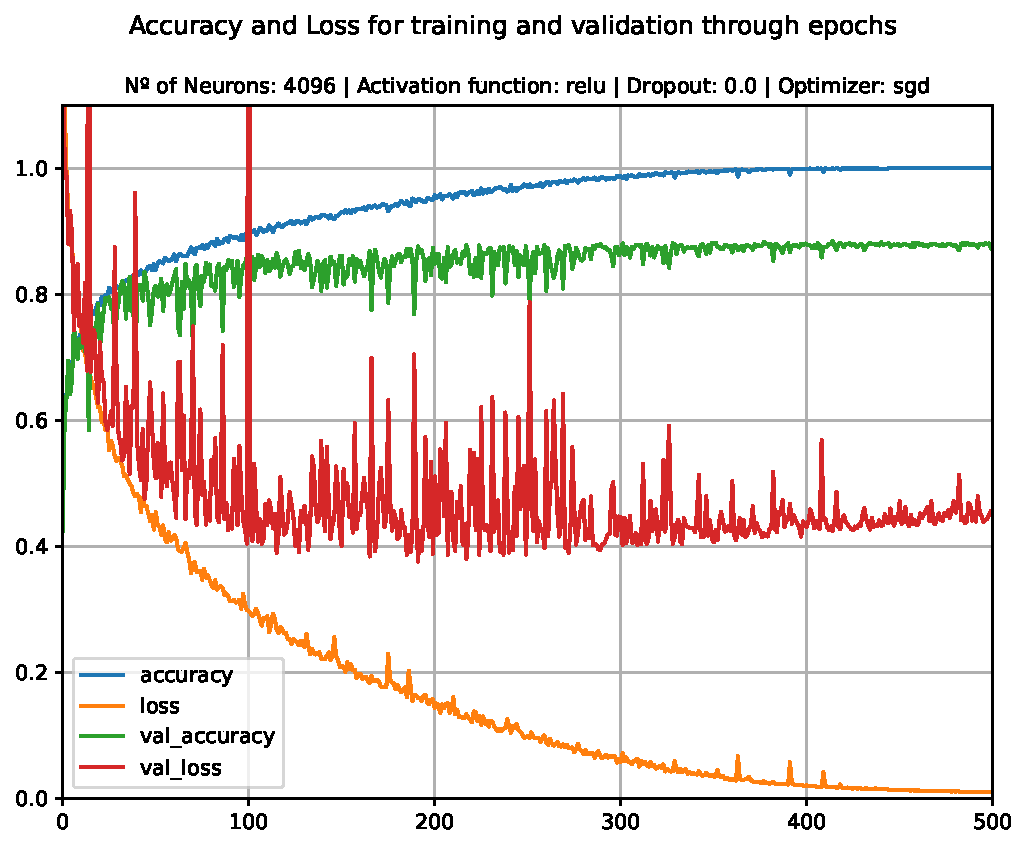
\includegraphics[width = \textwidth]{../../plot/mlp/mlp_4096_relu_0.0_sgd}
		\caption{ReLU.}
		\label{fig:mlp_4096_relu_0.0_sgd_act_fnc}
	\end{subfigure}
	\begin{subfigure}[H]{0.49\textwidth}
		\centering
		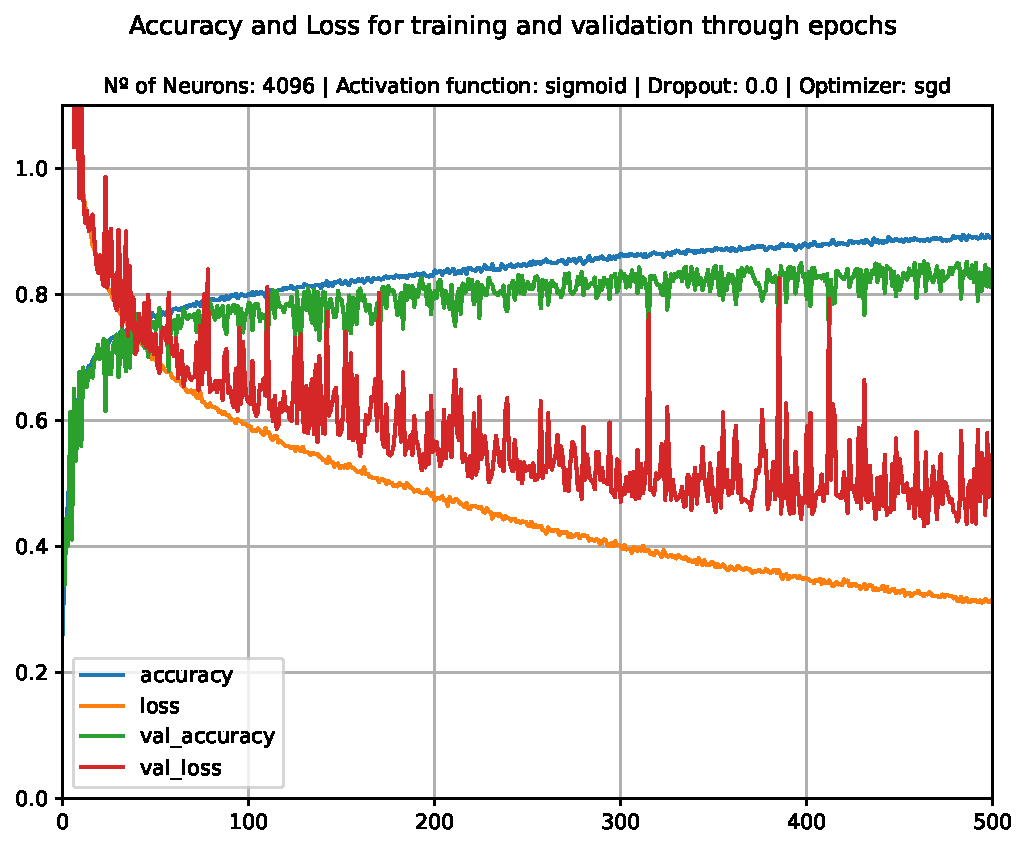
\includegraphics[width = \textwidth]{../../plot/mlp/mlp_4096_sigmoid_0.0_sgd}
		\caption{Sigmoide.}
		\label{fig:mlp_4096_sigmoid_0.0_sgd}
	\end{subfigure}
	\caption{Evolução da perda e acurácia de treinamento e validação com as épocas de treinamento para cada função de ativação candidata.}
\end{figure}

Como previsto pelos dados de treinamento, a acurácia para a rede com função de ativação logística é menor, como visto na \autoref{fig:search_activation_fnc}. Dessa forma, a função ReLU foi mantida como função de ativação do modelo final, e continuará sendo usada nas próximas buscas.

\begin{figure}[H]
\centering
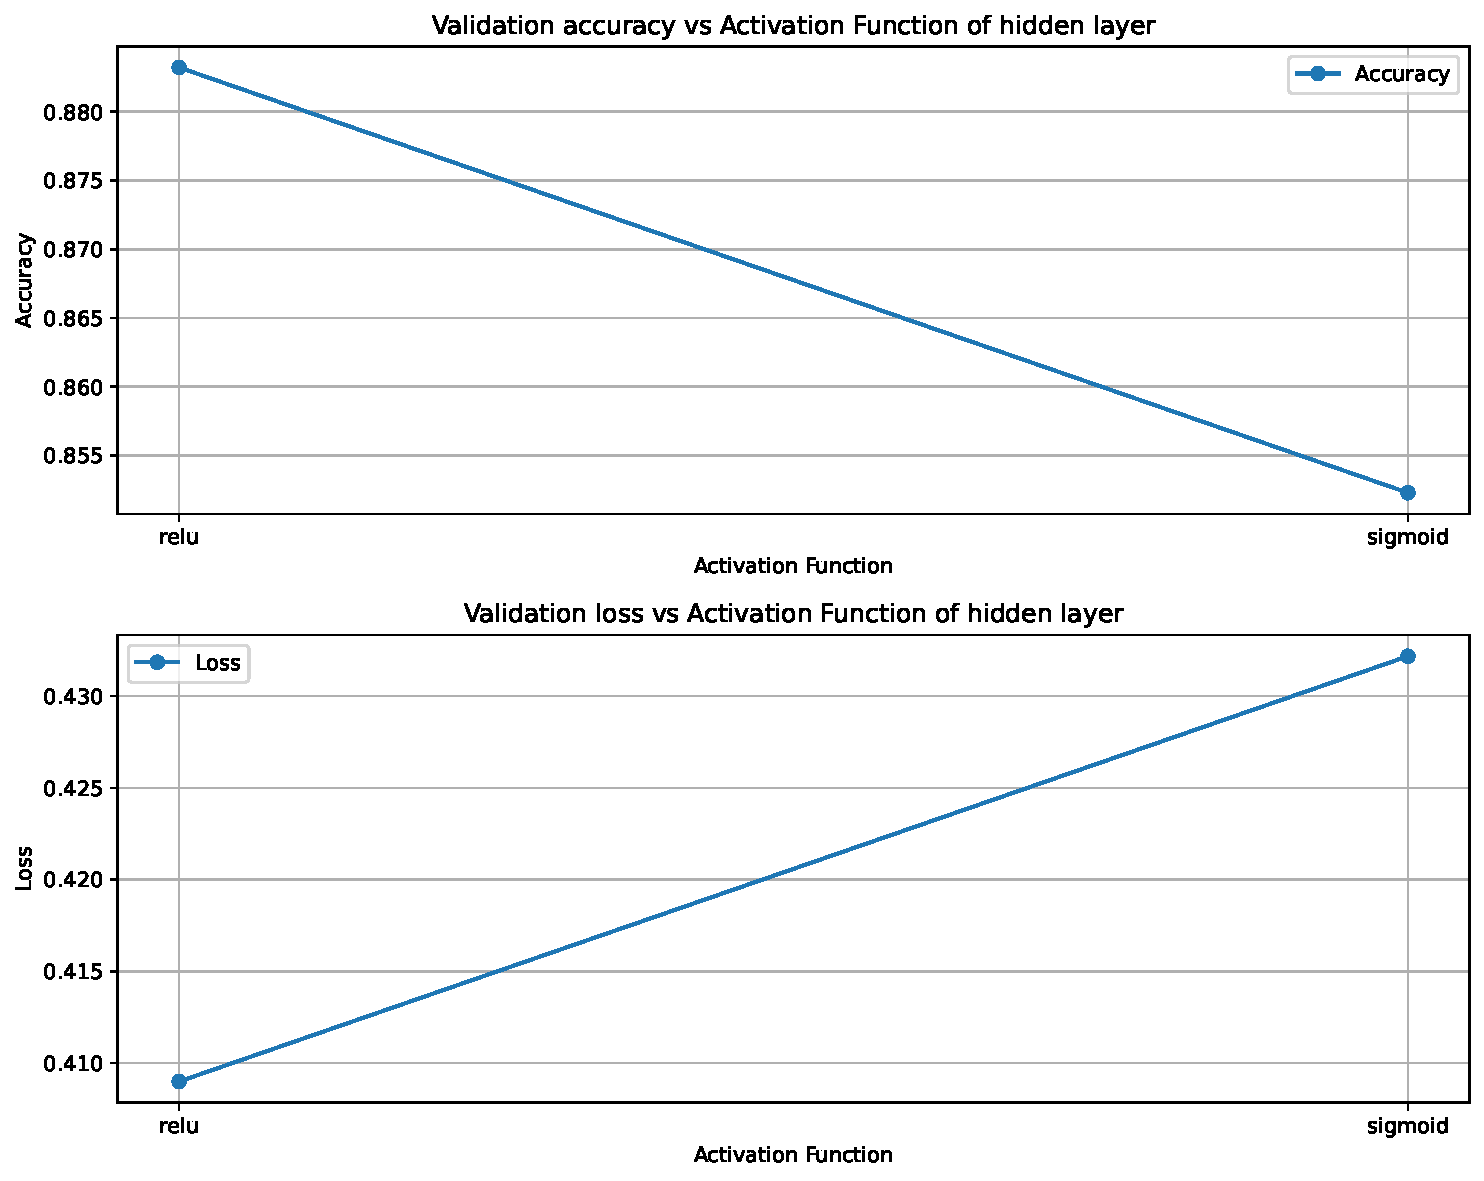
\includegraphics[width=0.75\linewidth]{../../plot/mlp/search_activation_fnc}
\caption{Acurácia e perda com a variação da função de ativação dos neurônios da camada intermediária.}
\label{fig:search_activation_fnc}
\end{figure}

\subsubsection{\textit{Dropout}}

	Uma vez que se está sendo utilizada uma rede com 4096 neurônios na camada intermediária, o treinamento se torna desafiador, onde para maximizar a capacidade de generalização, se deseja que todos os neurônios apresentem uma função útil na camada. Para isso, buscou-se o uso do \textit{dropout}, que foi testado com diferentes taxas.
	
	Os gráficos da \autoref{fig:training_search_dropout} mostram a evolução do treinamento da MLP sem \textit{dropout}, e com taxas de \textit{dropout} de 0,25 e 0,5. Observa-se primeiramente, que a inserção dessa técnica limitou o \textit{overfitting}, e para o caso da \autoref{fig:mlp_4096_relu_0.5_sgd}, resultou em uma maior lentidão do treinamento da rede, ou seja, o desligamento dos neurônios se tornou forte o suficiente para diminuir a capacidade de aprendizado da rede.
	

\begin{figure}[H]
	\centering
	\begin{subfigure}[H]{0.49\textwidth}
		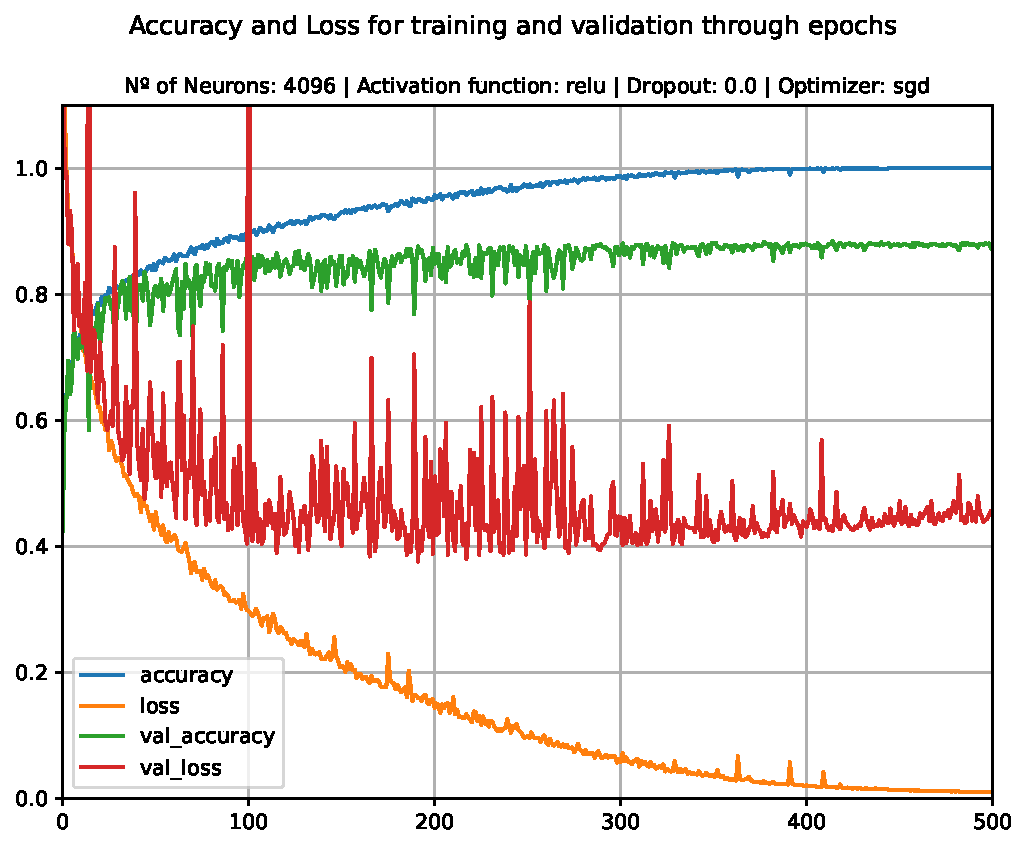
\includegraphics[width = \textwidth]{../../plot/mlp/mlp_4096_relu_0.0_sgd}
		\caption{0,0.}
		\label{fig:mlp_4096_relu_0.0_sgd_dropout}
	\end{subfigure}
	\begin{subfigure}[H]{0.49\textwidth}
		\centering
		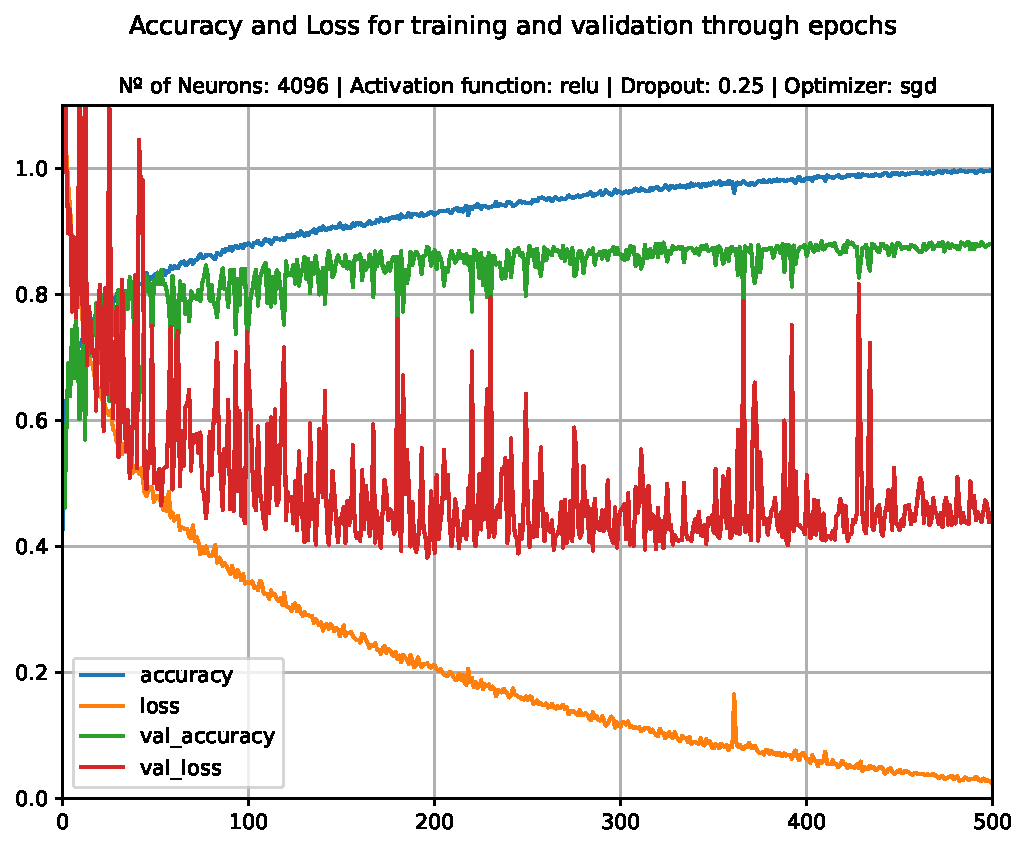
\includegraphics[width = \textwidth]{../../plot/mlp/mlp_4096_relu_0.25_sgd}
		\caption{0,25.}
		\label{fig:mlp_4096_relu_0.25_sgd}
	\end{subfigure}
	\begin{subfigure}[H]{0.49\textwidth}
		\centering
		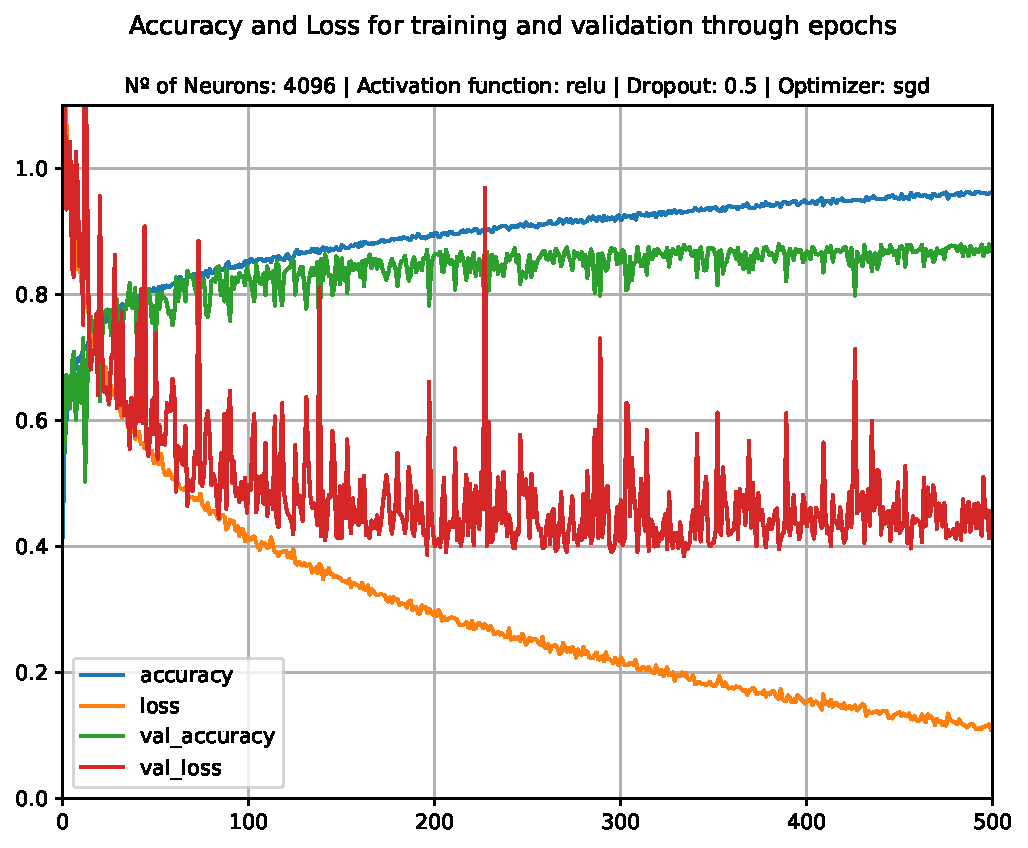
\includegraphics[width = \textwidth]{../../plot/mlp/mlp_4096_relu_0.5_sgd}
		\caption{0,5.}
		\label{fig:mlp_4096_relu_0.5_sgd}
	\end{subfigure}
	\caption{Evolução da perda e acurácia de treinamento e validação com as épocas de treinamento para diferentes taxas de \textit{dropout}.}
	\label{fig:training_search_dropout}
\end{figure}

Dessa forma, a taxa de \textit{dropout} de 0,25 foi incorporada à rede MLP, e será utilizada nas buscas posteriores.

\begin{figure}[H]
\centering
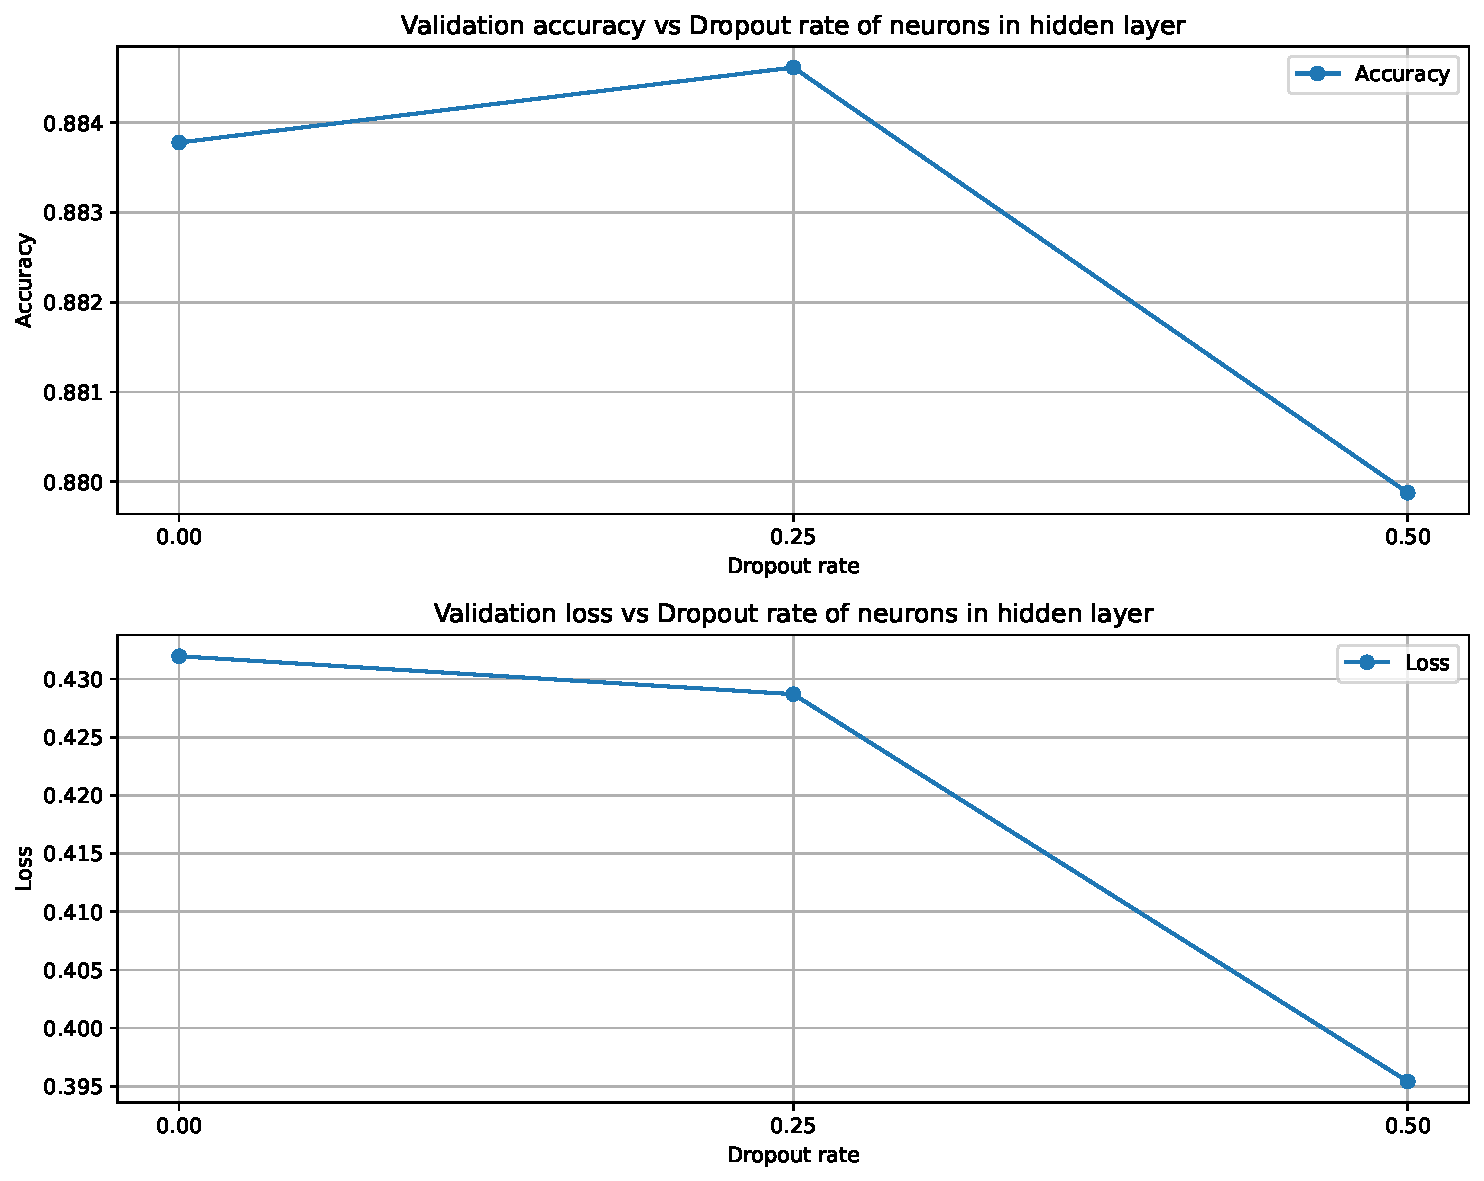
\includegraphics[width=0.75\linewidth]{../../plot/mlp/search_dropout}
\caption{Acurácia e perda com a variação da taxe de \textit{dropout} dos neurônios da camada intermediária.}
\label{fig:search_dropout}
\end{figure}

\subsubsection{Otimizador}

	Uma vez que a superfície de erro é desconhecida e comumente multimodal, o uso de um bom otimizador se faz crucial para garantir a convergência do modelo para um bom mínimo local, que garante uma melhor chance de maximização da capacidade de generalização do modelo. Para a busca, foram candidatos um algoritmo clássico, o \textit{Stochastic Descendent Gradient} (SGD), e um algoritmo adaptativo, o ADAM. 
	
	O treinamento com cada um dos otimizadores se dá na \autoref{fig:train_search_opt}, onde pode-se observar que como esperado, o algoritmo adaptativo converge em menos épocas e de forma menos ruidosa, porém para um mínimo local de pior qualidade. Já o SGD, apresenta uma trajetória ruidosa, mas consegue alcançar um mínimo local de melhor qualidade, atingindo valores altos de acurácia e minimizando consideravelmente a perda.

\begin{figure}[H]
	\centering
	\begin{subfigure}[H]{0.49\textwidth}
		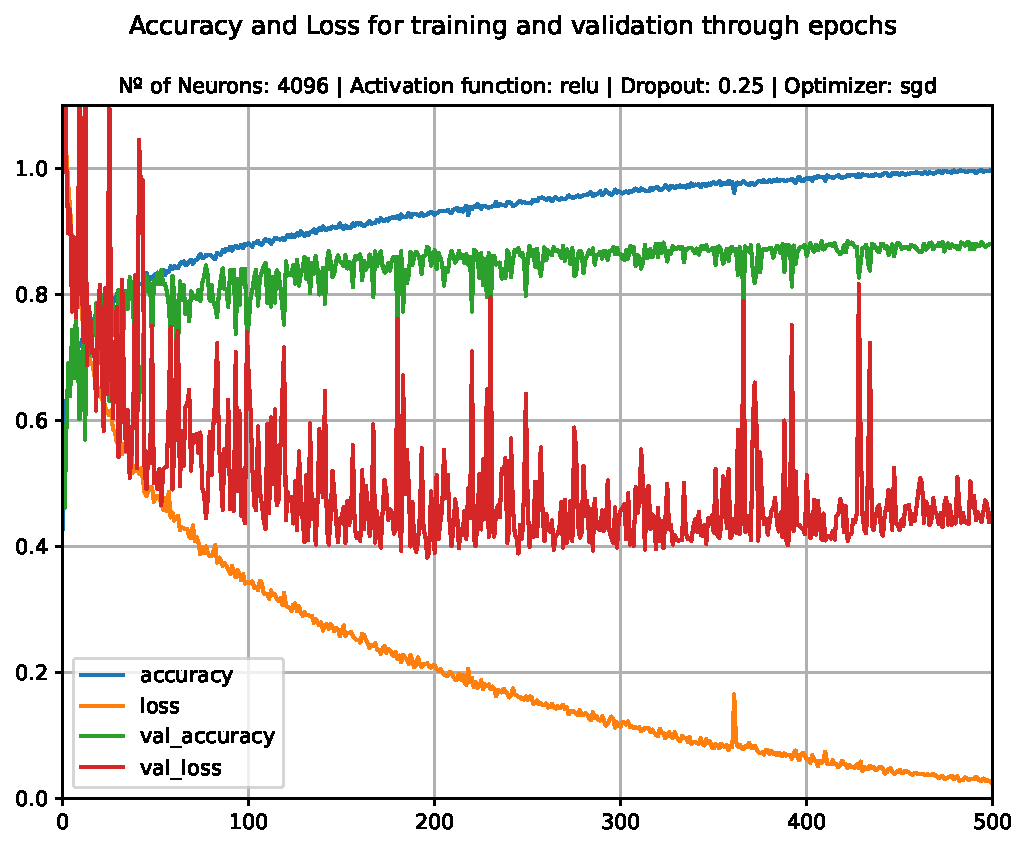
\includegraphics[width = \textwidth]{../../plot/mlp/mlp_4096_relu_0.25_sgd}
		\caption{ReLU.}
		\label{fig:mlp_4096_relu_0.0_sgd_opt}
	\end{subfigure}
	\begin{subfigure}[H]{0.49\textwidth}
		\centering
		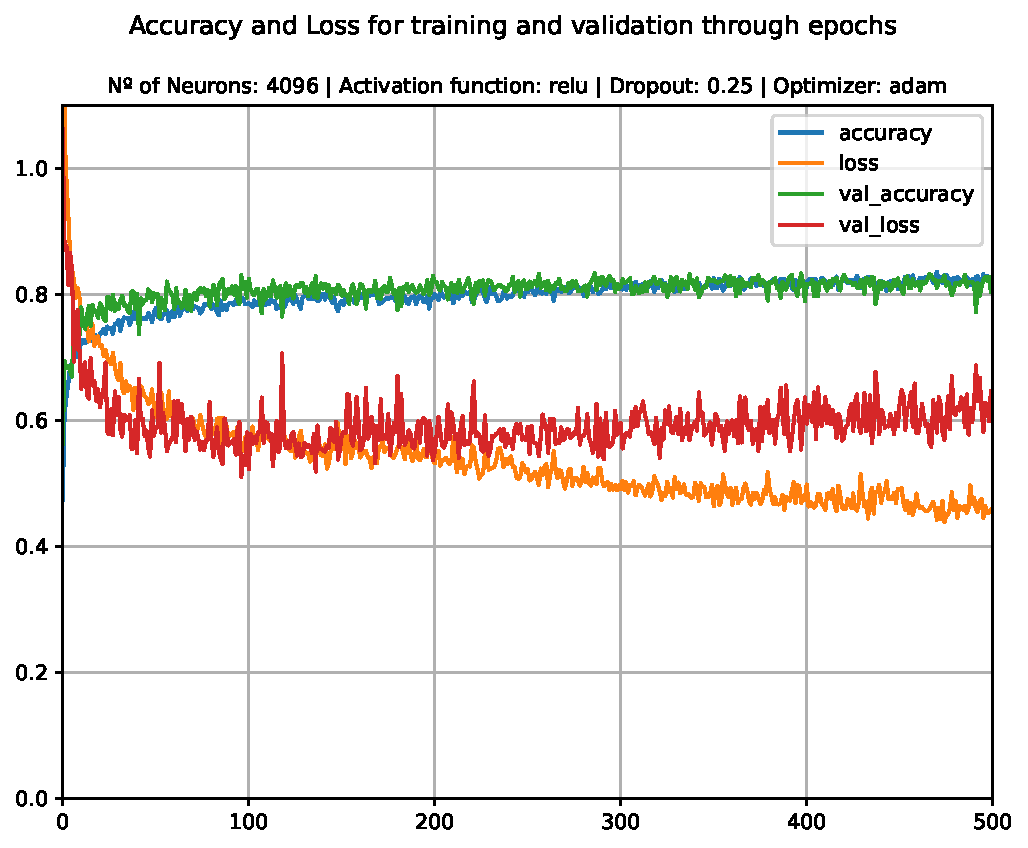
\includegraphics[width = \textwidth]{../../plot/mlp/mlp_4096_relu_0.25_adam}
		\caption{Sigmoide.}
		\label{fig:mlp_4096_relu_0.25_adam}
	\end{subfigure}
	\caption{Evolução da perda e acurácia de treinamento e validação com as épocas de treinamento para os otimizadores analisados.}
	\label{fig:train_search_opt}
\end{figure}

	Como já se sabe, algoritmos adaptativos tendem a convergir em menos épocas, porém nada se garante sobre a qualidade do mínimo local de convergência. No trabalho realizado por \citeonline{wilson2018marginal}, a principal conclusão obtida é que máquinas treinadas com algoritmos adaptativos tendem a generalizar pior do que máquinas treinadas com algoritmos de SGD. Dessa forma, o mesmo resultado pode ser visto na MLP treinada, onde pela \autoref{fig:search_optimizer}, observa-se que a rede neural treinada com SGD consegue uma acurácia consideravelmente maior, e minimiza mais a função de custo sobre os dados de validação.
	
	Sendo assim, o algoritmo de otimização SGD foi definido para o modelo final da rede, encerrando a busca de hiper-parâmetros.

\begin{figure}[H]
\centering
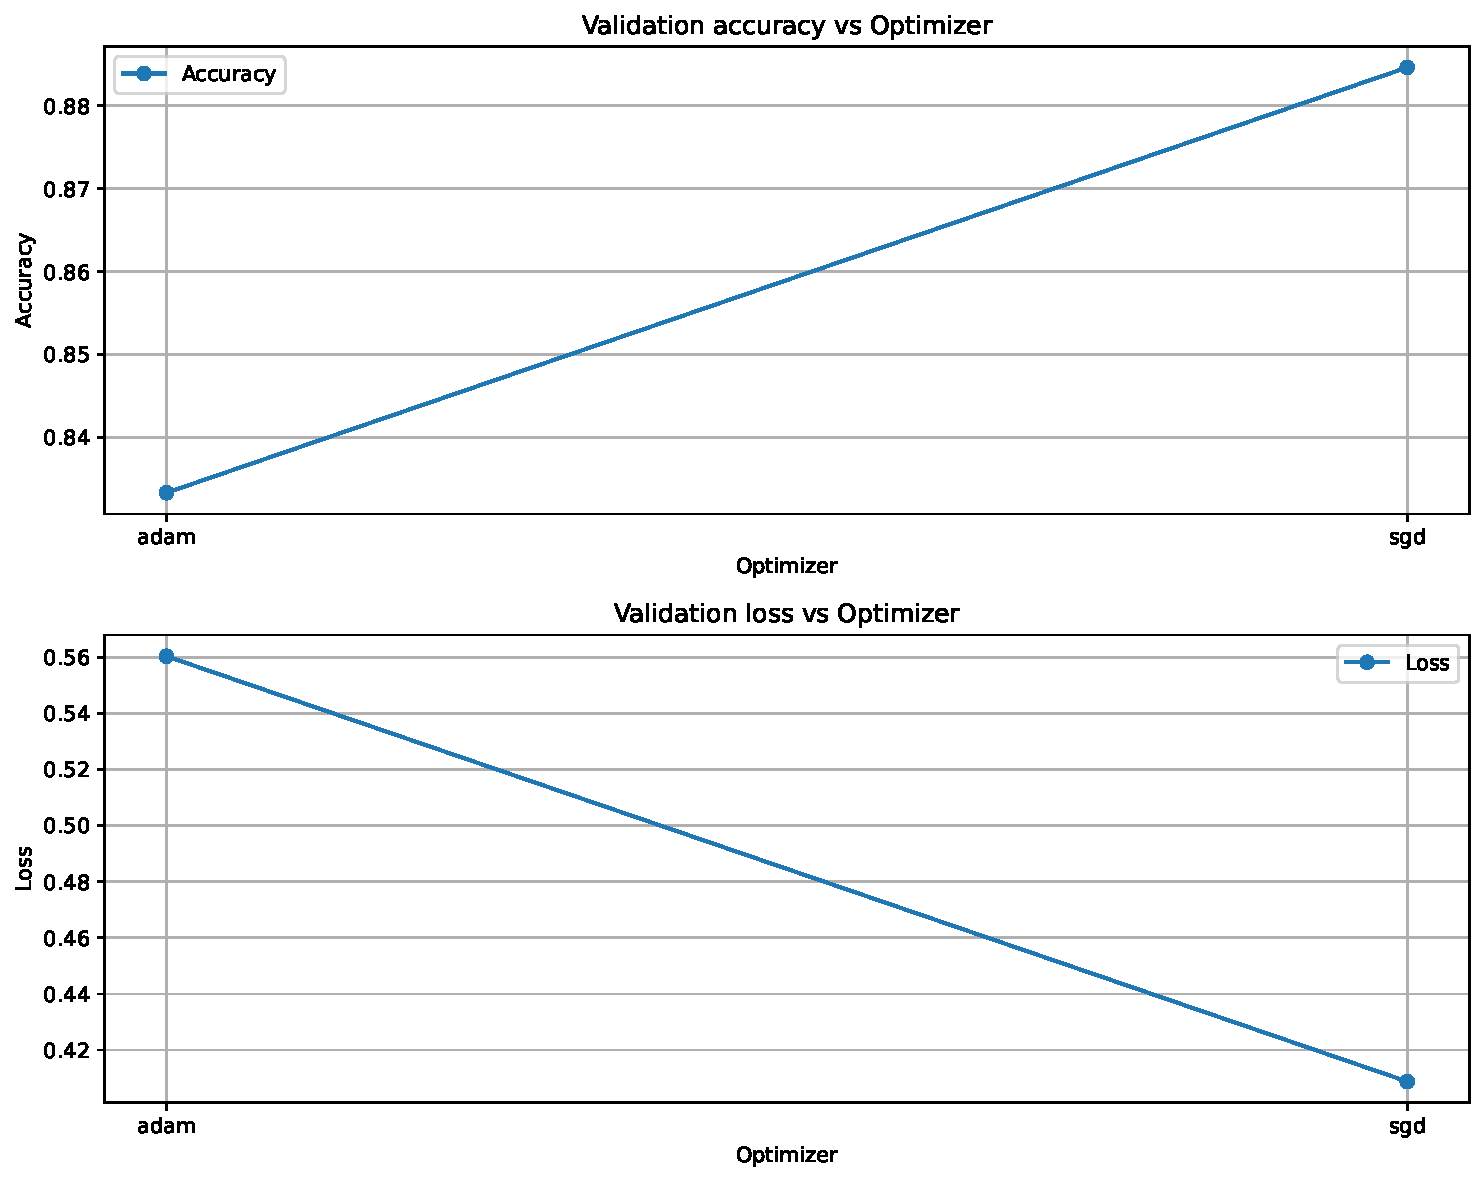
\includegraphics[width=0.65\linewidth]{../../plot/mlp/search_optimizer}
\caption{Acurácia e perda com a variação do algoritmo de otimização.}
\label{fig:search_optimizer}
\end{figure}

\subsection{Análise do melhor modelo}

	Com a realização da busca exaustiva, foram obtidos como melhores hiper-parâmetros para a rede MLP: 
	
	\begin{itemize}
		\item Número de neurônios: [ \texttt{4096} ]
		\item Função de ativação: [ \texttt{ReLU} ]
		\item \textit{Dropout}: [ \texttt{0,25} ]
		\item Otimizador: [ \texttt{SGD} ]
	\end{itemize} 

	Essa rede apresenta um total de 9,670,664 pesos treináveis, que uma vez ajustados durante o treinamento, apresentaram os seguintes valores de acurácia e acurácia balanceada frente aos dados de teste:

\begin{equation}\label{eq:acc_MLP}
	Accuracy = 0.8705
\end{equation}

\begin{equation}\label{eq:ba_MLP}
	BA = 0.8437
\end{equation}

	A matriz de confusão do classificador é exibida na \autoref{tab:mc_MLP}. Primeiramente, observa-se que a classe 3 é a mais desafiadora, uma vez que ela é fortemente confundida com as classes 0, 2, 4, 5 e 6, sendo a classe 7 a única que não se confunde com a 3. Pela \autoref{tab:pr_MLP}, consegue-se ter um melhor panorama da precisão e do \textit{recall} das classes, uma vez que as mesmas não são balanceadas. Como esperado, a classe 3 apresenta baixa precisão e o pior \textit{recall}, mas a classe 0 é a que apresenta pior precisão, apresentando falsos positivos para a classe 3, 4 e 5. A classe 7 é a que apresenta a melhor classificação, com precisão quase unitária.


\begin{table}[H]
	\centering
	\begin{tabular}{c||c|c|c|c|c|c|c|c|}
		\cline{2-9}
		\textbf{}                        & \textbf{0} & \textbf{1} & \textbf{2} & \textbf{3} & \textbf{4} & \textbf{5} & \textbf{6} & \textbf{7} \\ \hline \hline
		\multicolumn{1}{|c||}{\textbf{0}} & 177        & 3          & 0          & 43         & 4          & 17         & 0          & 0          \\ \hline
		\multicolumn{1}{|c||}{\textbf{1}} & 1          & 613        & 0          & 3          & 1          & 0          & 6          & 0          \\ \hline
		\multicolumn{1}{|c||}{\textbf{2}} & 4          & 1          & 264        & 16         & 6          & 3          & 11         & 6          \\ \hline
		\multicolumn{1}{|c||}{\textbf{3}} & 34         & 26         & 3          & 447        & 5          & 32         & 32         & 0          \\ \hline
		\multicolumn{1}{|c||}{\textbf{4}} & 13         & 0          & 11         & 31         & 182        & 0          & 6          & 0          \\ \hline
		\multicolumn{1}{|c||}{\textbf{5}} & 10         & 2          & 1          & 48         & 3          & 215        & 5          & 0          \\ \hline
		\multicolumn{1}{|c||}{\textbf{6}} & 0          & 22         & 5          & 22         & 2          & 2          & 611        & 2          \\ \hline
		\multicolumn{1}{|c||}{\textbf{7}} & 0          & 0          & 1          & 0          & 0          & 0          & 0          & 469        \\ \hline
	\end{tabular}
	\caption{Matriz de confusão do classificador baseado em MLP.}
	\label{tab:mc_MLP}
\end{table}

\begin{table}[H]
\centering
\begin{tabular}{c|c|c}
	\textbf{Classe} & \textbf{Precisão} & \textit{\textbf{Recall}} \\ \hline
	\textbf{0}     & 0.7254            & 0.7406                   \\
	\textbf{1}     & 0.9824            & 0.9190                   \\
	\textbf{2}     & 0.8489            & 0.9263                   \\
	\textbf{3}     & 0.7720            & 0.7328                   \\
	\textbf{4}     & 0.7490            & 0.8966                   \\
	\textbf{5}     & 0.7570            & 0.7993                   \\
	\textbf{6}     & 0.9174            & 0.9106                   \\
	\textbf{7}     & 0.9979            & 0.9832                  
\end{tabular}
\caption{Precisão e \textit{recall} por classe do classificador baseado em MLP.}
\label{tab:pr_MLP}
\end{table}

\subsubsection{Análise dos erros}

Foram selecionados alguns casos de erro, onde é exibido a amostra que foi classificada erroneamente, uma representante da classe do falso positivo, e uma representante da classe real daquela amostra, seguido pelas probabilidades daquele dado pertencer a cada uma das classes.

Nas Figuras~\ref{fig:error_analyser_88}~e~\ref{fig:error_analyser_36}, observa-se que houve grande desafio para classificar a classe da amostra, e a classe correta se encontra como a 2ª maior probabilidade, sem estar consideravelmente para trás.

\begin{figure}[H]
\centering
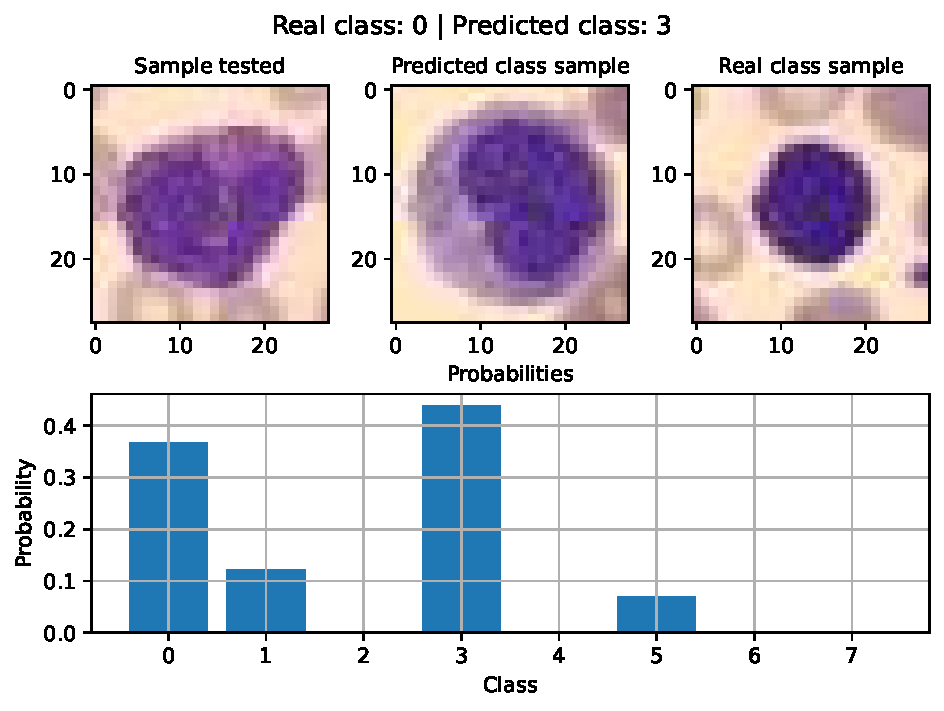
\includegraphics[width=0.75\linewidth]{../../plot/mlp/error_analyser_88}
\caption{Análise de um caso de erro de classificação.}
\label{fig:error_analyser_88}
\end{figure}

\begin{figure}[H]
\centering
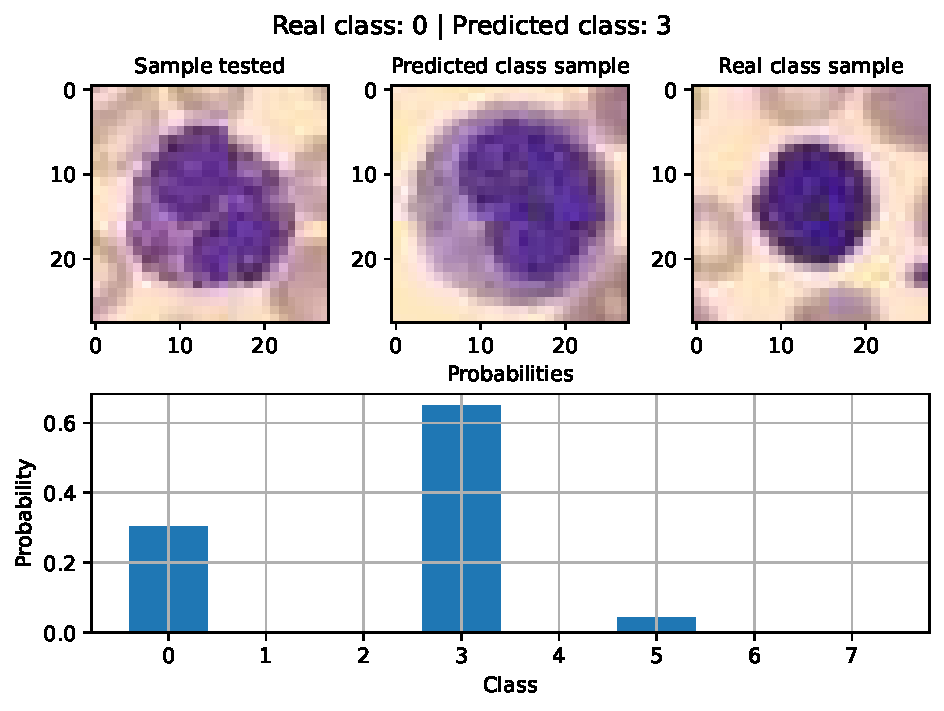
\includegraphics[width=0.75\linewidth]{../../plot/mlp/error_analyser_36}
\caption{Análise de um caso de erro de classificação.}
\label{fig:error_analyser_36}
\end{figure}

Já para as amostras das Figuras~\ref{fig:error_analyser_0}~e~\ref{fig:error_analyser_62}, o classificador errou com grande certeza, apresentando mais de 0,8 de probabilidade de ser a classe errada, mostrando uma grande falha na classificação. Porém, a classe correta continuou sendo a 2ª mais provável.

\begin{figure}[H]
\centering
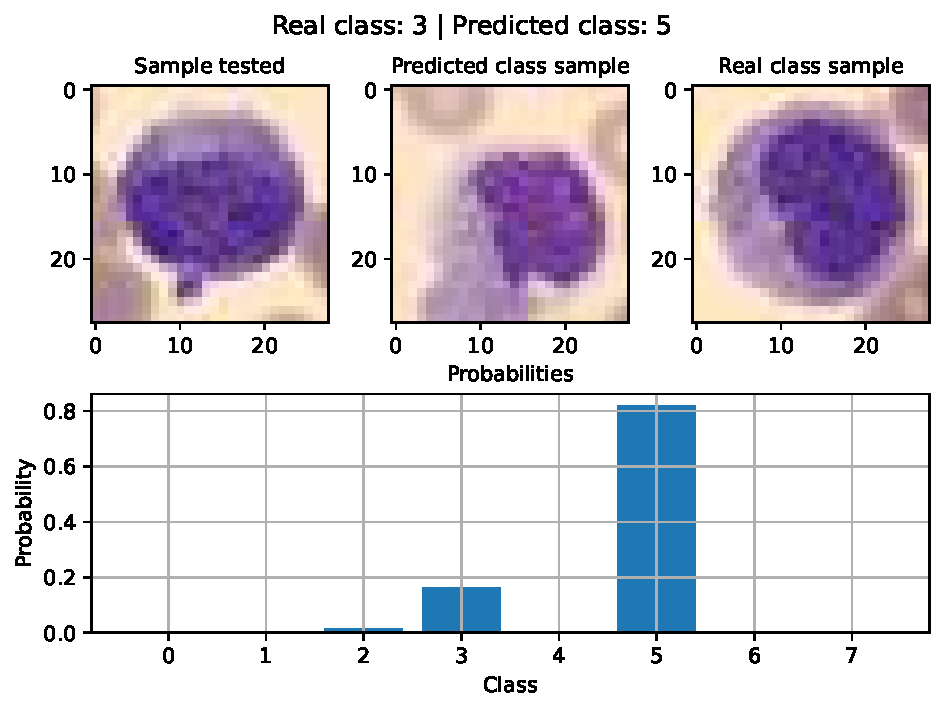
\includegraphics[width=0.75\linewidth]{../../plot/mlp/error_analyser_0}
\caption{Análise de um caso de erro de classificação.}
\label{fig:error_analyser_0}
\end{figure}

\begin{figure}[H]
\centering
\includegraphics[width=0.75\linewidth]{../../plot/mlp/error_analyser_62}
\caption{Análise de um caso de erro de classificação.}
\label{fig:error_analyser_62}
\end{figure}

Já para a classificação do dado da \autoref{fig:error_analyser_25}, houve grande certeza que a amostra era da classe 1, apresentando na sequência maiores probabilidades de pertencer à classe 2 e 7, respectivamente. Porém, a classe correta, 6, foi a 4ª mais provável, se mostrando como uma amostra muito desafiadora, o que pode ser percebido visualmente, por apresentar um padrão muito diferente do visto para a classe 6 na \autoref{fig:samples_of_classes}.

\begin{figure}[H]
\centering
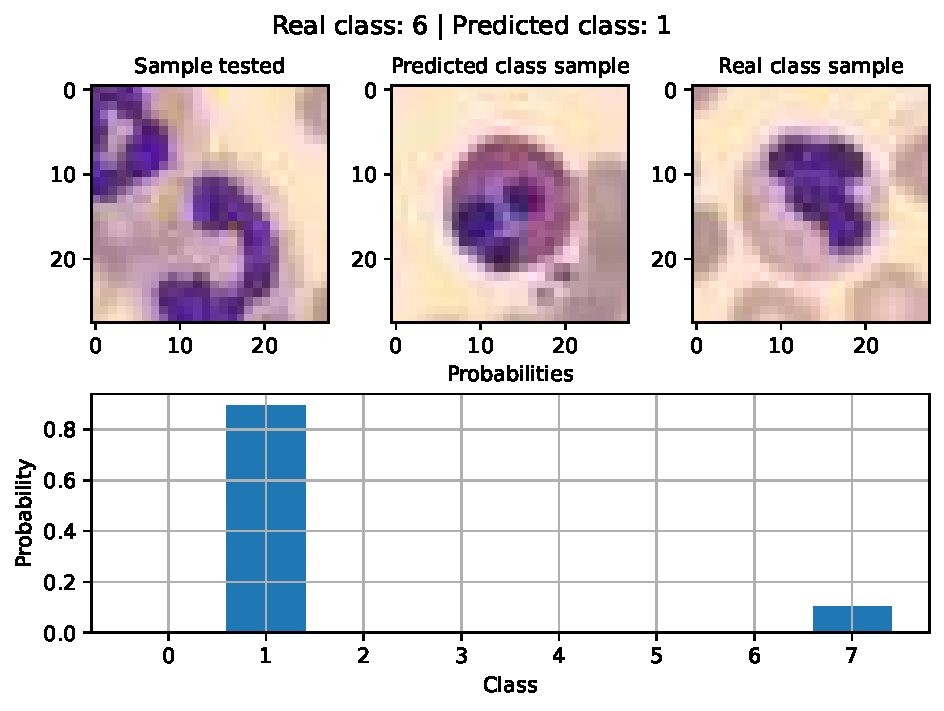
\includegraphics[width=0.75\linewidth]{../../plot/mlp/error_analyser_25}
\caption{Análise de um caso de erro de classificação.}
\label{fig:error_analyser_25}
\end{figure}




%%%%%%%%%%%%%%%%%%%%%%%%%%%%%%%%%%%%%%%%%%%%%%%%%%%%%%%%%%%%%%%%%%%%%%%%%%%%%%
\clearpage
\section{CNN Simples}

Para a implementação a rede neural convolucional (CNN) com arquitetura rasa (\textit{shallow}), foi utilizada uma rede possuindo apenas uma camada convolucional, uma camada de \textit{pooling} e uma camada de saída com função de ativação \textit{softmax}.

Com base no visto anteriormente, a função de ativação foi mantida como ReLU, o otimizador como SGD e não foi empregado o uso de \textit{dropout}, devido ao tamanho da rede. A camada de \textit{pooling} escolhida utiliza a operação de máximo, operação selecionada a partir de um teste prévio, que mostrou maior acurácia da rede utilizando a operação de máximo frente à operação de média. O \textit{kernel} de \textit{pooling} foi mantido em um tamanho pequeno, de 2x2, pois como a rede é rasa, houve a intenção de preservar a maior quantidade de dados possível, em vista que não há expansão do campo receptivo.

\subsection{Busca do melhor modelo}

Para realizar a busca do melhor modelo de CNN, foram treinadas redes para os números de \textit{kernels} e tamanhos de \textit{kernels} mostrados a seguir:

\begin{itemize}
	\item Número de \textit{kernels}: [ \texttt{8}; \texttt{16}; \texttt{32}; \texttt{64}; \texttt{128} ]
	\item Tamanho dos \textit{kernels}: [ \texttt{3x3}; \texttt{5x5}; \texttt{7x7}; \texttt{9x9} ]
\end{itemize}

Diferentemente da MLP, devido à variação de somente dois hiper-parâmetros, foi realizada a busca exaustiva completa sobre tais variáveis no intervalo estipulado, e o mesmo foi expresso em um gráfico de temperatura, mostrado na \autoref{fig:hiper_parameters_search}. Observa-se que a acurácia aumenta com o aumento do número de \textit{kernels}, e também com o aumento do tamanho do \textit{kernel}, mas principalmente com o primeiro. Como a rede convolucional possuí apenas uma camada convolucional, não existe a expansão do campo receptivo dos neurônios sob o dado de entrada através das camadas, logo, um \textit{kernel} maior consegue captar mais padrões, e dessa forma, chegar à um desempenho melhor. Já em relação ao número de \textit{kernels}, é esperado que possuindo mais canais, cada canal possa detectar um atributo diferente e dessa forma generalizar melhor.

Devido ao pouco ganho de acurácia da configuração com \textit{kernel} 9x9 para 64 ou 128 \textit{kernels}, escolheu-se a opção com menos \textit{kernels} para simplicidade da CNN, obtendo assim o melhor configuração da CNN \textit{Shallow}: 

\begin{itemize}
	\item Número de \textit{kernels}: [ \texttt{64} ]
	\item Tamanho dos \textit{kernels}: [ \texttt{9x9} ]
\end{itemize}

\begin{figure}[H]
\centering
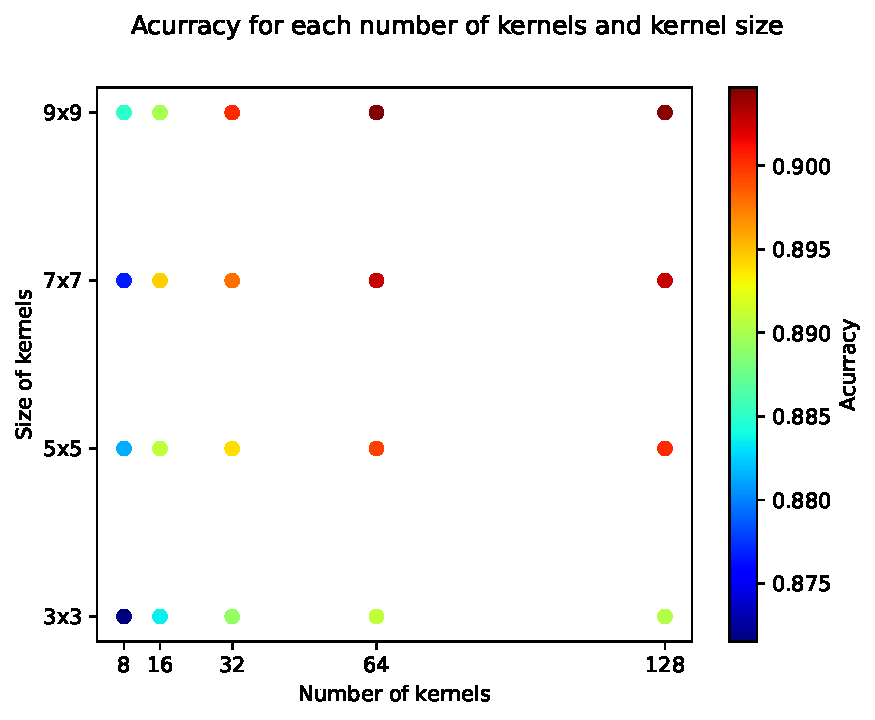
\includegraphics[width=0.75\linewidth]{../../plot/cnn_shallow/hiper_parameters_search}
\caption{Acurácia do classificador de acordo com o número e tamanho dos \textit{kernels}.}
\label{fig:hiper_parameters_search}
\end{figure}

A \autoref{fig:best_model_training} mostra o treinamento da rede com melhor configuração por 200 épocas. Observa-se que a perda sob os dados de validação é bem menos errática, e não se percebe \textit{overfitting}. Devido à saturação da acurácia, se fez satisfatório o treinamento em apenas 200 épocas, adotando de \textit{early stopping} para concluir o treinamento da rede.

\begin{figure}[H]
\centering
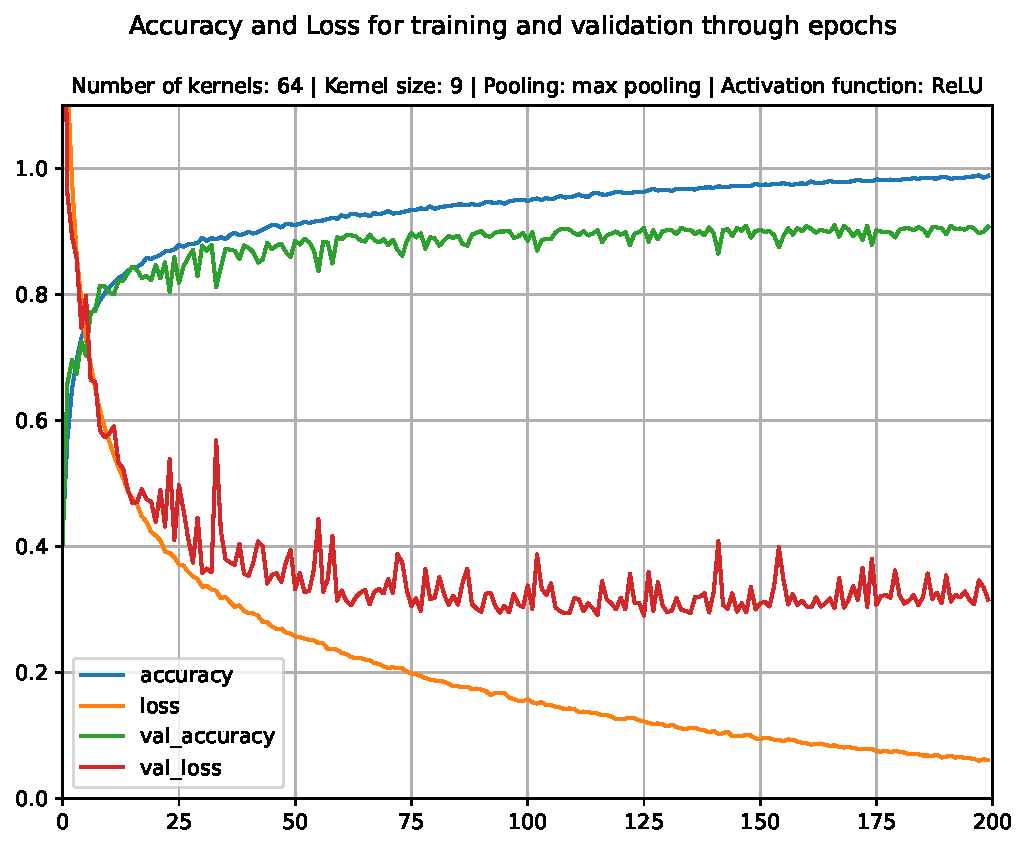
\includegraphics[width=0.65\linewidth]{../../plot/cnn_shallow/best_model_training}
\caption{Acurácia e perda durante as épocas de treinamento do melhor modelo CNN \textit{Shallow}.}
\label{fig:best_model_training}
\end{figure}

\subsection{Análise do Melhor modelo}

	Avaliando o desempenho do modelo com melhor configuração, o primeiro contraste que se explicita é que ele possuí apenas 115,976 pesos treináveis, uma quantidade drasticamente inferior à da rede com camada densa. A acurácia e acurácia balanceada do classificador se veem em \eqref{eq:accuracy_CNN_shallow} e \eqref{eq:BA_CNN_shallow}, apresentando um desempenho superior ao da MLP, com uma quantidade 842 vezes menor de parâmetros.

\begin{equation}\label{eq:accuracy_CNN_shallow}
	Accuracy = 0.9088
\end{equation}

\begin{equation}\label{eq:BA_CNN_shallow}
	BA = 0.8905
\end{equation}

A matriz de confusão do classificador baseado em CNN \textit{Shallow} se encontra na \autoref{tab:mc_CNN_shallow}.

\begin{table}[H]
	\centering
	\begin{tabular}{c||c|c|c|c|c|c|c|c|}
		\cline{2-9}
		\textbf{}                        & \textbf{0} & \textbf{1} & \textbf{2} & \textbf{3} & \textbf{4} & \textbf{5} & \textbf{6} & \textbf{7} \\ \hline \hline
		\multicolumn{1}{|c||}{\textbf{0}} & 193        & 2          & 1          & 34         & 4          & 10         & 0          & 0          \\ \hline
		\multicolumn{1}{|c||}{\textbf{1}} & 2          & 610        & 0          & 4          & 1          & 1          & 6          & 0          \\ \hline
		\multicolumn{1}{|c||}{\textbf{2}} & 3          & 2          & 286        & 9          & 2          & 3          & 4          & 2          \\ \hline
		\multicolumn{1}{|c||}{\textbf{3}} & 23         & 12         & 14         & 478        & 13         & 21         & 18         & 0          \\ \hline
		\multicolumn{1}{|c||}{\textbf{4}} & 9          & 0          & 6          & 12         & 214        & 1          & 1          & 0          \\ \hline
		\multicolumn{1}{|c||}{\textbf{5}} & 4          & 0          & 4          & 50         & 6          & 219        & 1          & 0          \\ \hline
		\multicolumn{1}{|c||}{\textbf{6}} & 1          & 7          & 2          & 14         & 2          & 0          & 640        & 0          \\ \hline
		\multicolumn{1}{|c||}{\textbf{7}} & 0          & 0          & 0          & 0          & 0          & 0          & 1          & 469        \\ \hline
	\end{tabular}
	\caption{Matriz de confusão do classificador baseado em CNN \textit{Shallow}.}
	\label{tab:mc_CNN_shallow}
\end{table}

\begin{table}[H]
	\centering
	\begin{tabular}{c|c|c}
		\textbf{Classe} & \textbf{Precisão} & \textit{\textbf{Recall}} \\ \hline
		\textbf{0}      & 0.7910            & 0.8213                   \\
		\textbf{1}      & 0.9776            & 0.9637                   \\
		\textbf{2}      & 0.9196            & 0.9137                   \\
		\textbf{3}      & 0.8256            & 0.7953                   \\
		\textbf{4}      & 0.8807            & 0.8843                   \\
		\textbf{5}      & 0.7711            & 0.8588                   \\
		\textbf{6}      & 0.9610            & 0.9538                   \\
		\textbf{7}      & 0.9979            & 0.9958                  
	\end{tabular}
	\caption{Matriz de confusão do classificador baseado em CNN \textit{Shallow}.}
	\label{tab:pr_CNN_shallow}
\end{table}

\subsubsection{Análise dos erros}

\begin{figure}[H]
\centering
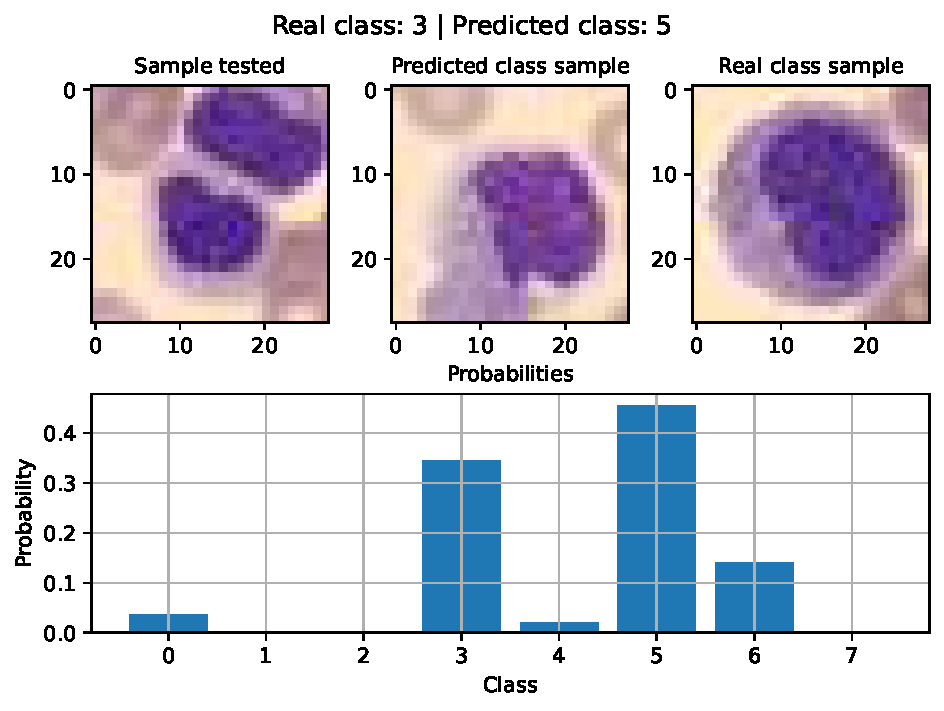
\includegraphics[width=0.75\linewidth]{../../plot/cnn_shallow/error_analyser_1455}
\caption{Análise de um caso de erro de classificação.}
\label{fig:error_analyser_1455}
\end{figure}

\begin{figure}[H]
\centering
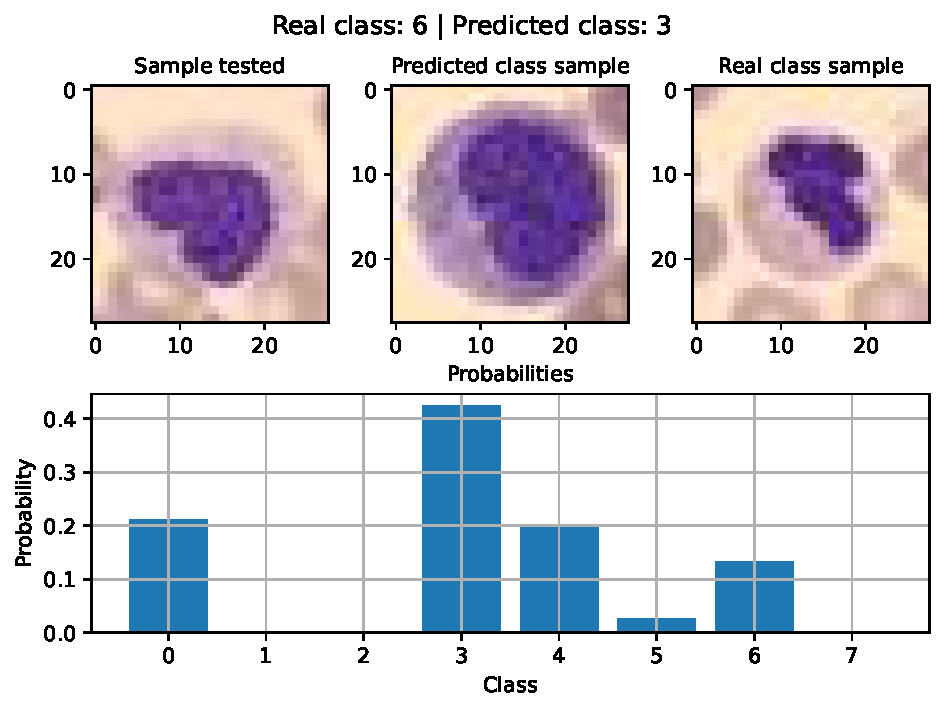
\includegraphics[width=0.75\linewidth]{../../plot/cnn_shallow/error_analyser_35}
\caption{Análise de um caso de erro de classificação.}
\label{fig:error_analyser_35}
\end{figure}

\begin{figure}[H]
\centering
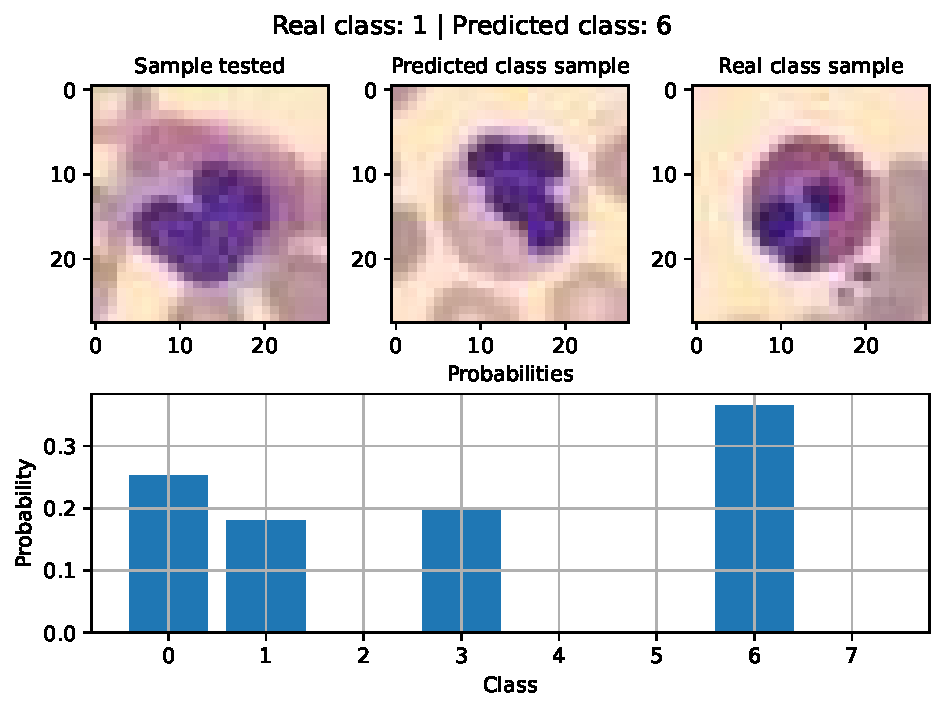
\includegraphics[width=0.75\linewidth]{../../plot/cnn_shallow/error_analyser_1516}
\caption{Análise de um caso de erro de classificação.}
\label{fig:error_analyser_1516}
\end{figure}

\begin{figure}[H]
\centering
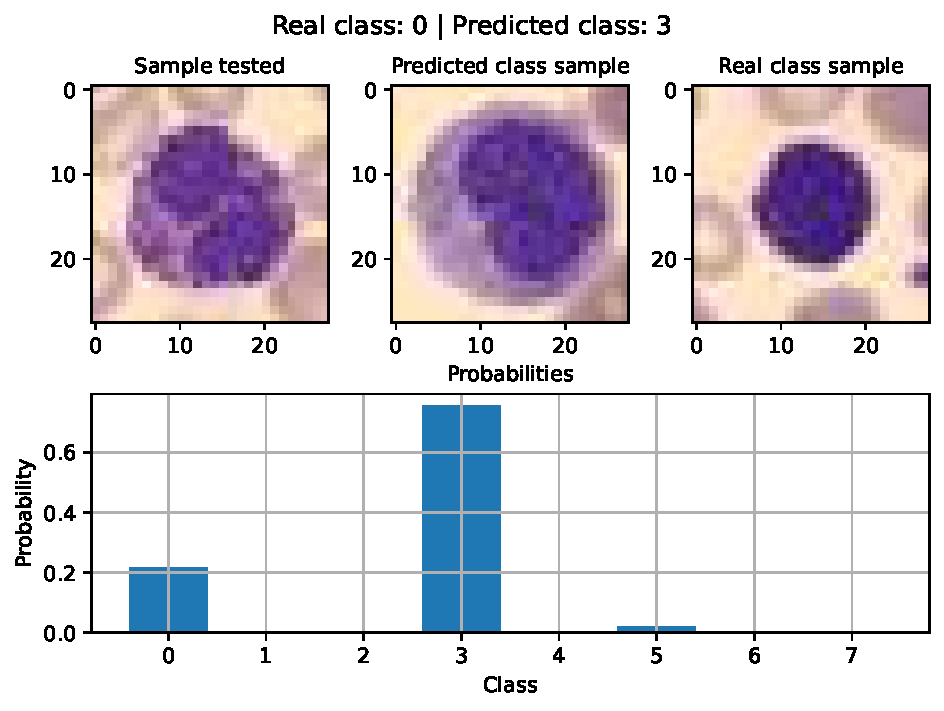
\includegraphics[width=0.75\linewidth]{../../plot/cnn_shallow/error_analyser_36}
\caption{Análise de um caso de erro de classificação.}
\label{fig:error_analyser_36_cnn}
\end{figure}

\begin{figure}[H]
\centering
\includegraphics[width=0.75\linewidth]{../../plot/cnn_shallow/error_analyser_62}
\caption{Análise de um caso de erro de classificação.}
\label{fig:error_analyser_62_cnn}
\end{figure}


\subsection{Aplicando uma entrada 64x64 à camada convolucional}

Como se sabe, a camada convolucional é robusta à alteração da dimensão do dado de entrada, ou seja, a rede aqui treinada para dados 28x28, suporta o processamento de dados de dimensão, como será testado, 64x64. Porém, como uma entrada maior gera \textit{feature maps} de saída também maiores, a camada convolucional terá seus pesos congelados, e uma nova camada de saída \textit{softmax} será treinada.

Ao treinar os 524,296 pesos resultantes da camada \textit{softmax}, conservando os 15,616 pesos da camada convolucional, obteve-se o perfil de treinamento mostrado na \autoref{fig:64x64_model_training}, e a acurácia sobre os dados de teste  \eqref{eq:64x64}. Uma vez que apenas a camada de saída foi treinada, para um dado consideravelmente maior de entrada, a queda de acurácia não se faz tão grande, uma vez que para uma entrada com esse tamanho, além de pesos com diferença relevante, pode se fazer necessário o uso de \textit{kernels} maiores. 

\begin{equation}\label{eq:64x64}
	Accuracy = 0.8620
\end{equation}

\begin{figure}[H]
	\centering
	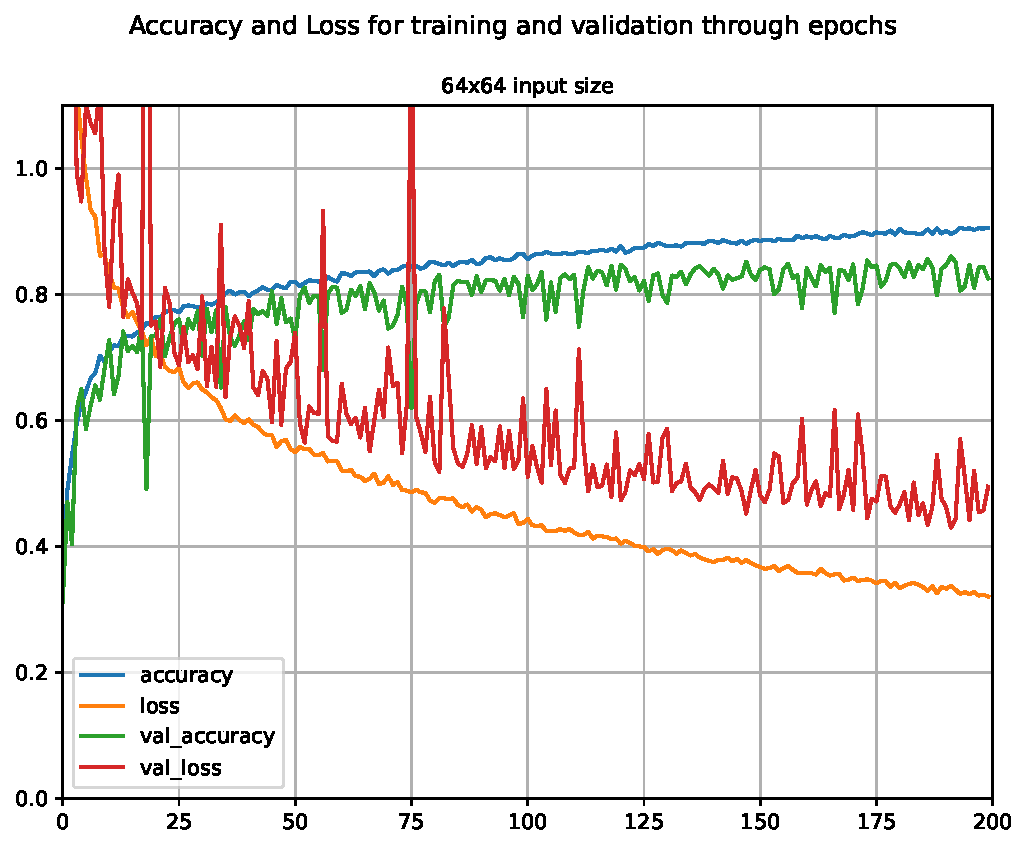
\includegraphics[width=0.75\linewidth]{../../plot/cnn_shallow/64x64_model_training}
	\caption{Análise de um caso de erro de classificação.}
	\label{fig:64x64_model_training}
\end{figure}


%%%%%%%%%%%%%%%%%%%%%%%%%%%%%%%%%%%%%%%%%%%%%%%%%%%%%%%%%%%%%%%%%%%%%%%%%%%%%%
\clearpage
\section{CNN Profunda}

Para a solução do problema de classificação das células sanguíneas, utilizando uma rede neural convolucional profunda, foi criada uma arquitetura inspirada nas \textit{DenseNets} \cite{huang2018densely}. A rede profunda modelo foi bastante simplificada, reduzindo o número de camadas, ao utilizar apenas um \textit{Dense Block}, e também considerando camadas convolucionais e de \textit{pooling} com \textit{stride} unitário, com intuito de preservar melhor a dimensão dos dados, em vista que a entrada utilizada é 28x28. Em vista disso, o tamanho do \textit{kernel} da camada de \textit{pooling} também foi alterada para 2x2, conservando um canal de saída maior, e a camada de transição não foi utilizada devido ao fato de não haver a concatenação de \textit{dense blocks}. A arquitetura da rede neural implementada é mostrada na \autoref{tab:cnn_dense}.

\begin{table}[H]
	\centering
	\begin{tabular}{c|c|cccc}
		\textbf{Camada}  & \textbf{Dimensão de saída} & \textbf{Descrição}                                                                                        \\ \hline
		Convolução       & $[28, \ 28, \ 3]$          & $128, \ 7\times 7 + 1(\text{S})$  + ReLU() + BN()                                                         \\ \hline
		\textit{Pooling} & $[14, \ 14, \ 64]$           & $\ 2\times 2 + 1(\text{S})$ max pooling                                                                   \\ \hline &&&\\[-1em]
		\textit{Dense Block}      & $[14, \ 14, \ 256]$        & $ \begin{bmatrix} 32, \ 1\times 1 + 1(\text{S}) \\ 32, \ 3\times 3 + 1(\text{S}) \end{bmatrix} + \text{ReLU}() + \text{BN}() \times 6 $ \\ &&&\\[-1em] \hline
		\textit{Pooling} & $[256]$                    & \textit{Global average pooling}                                                                         \\ \hline
		Saída            & $[8]$                      & \textit{softmax}()                                                                                                
	\end{tabular}
	\caption{Estrura da CNN profunda baseada na \textit{DenseNet}.}
	\label{tab:cnn_dense}
\end{table}

A rede possuí um total de 351,048 parâmetros, sendo 347,656 deles treináveis. Observa-se que mesmo com a camada densa de saída, o número de parâmetros não aumenta expressivamente devido ao uso da camada de \textit{global average pooling}, que compacta cada canal de saída do \textit{dense block} em um único valor, reduzindo consideravelmente a quantidade de dados que serão enfileirados para gerar a saída pela camada \textit{softmax}. 

\subsection{Análise do desempenho}

\begin{equation}\label{eq:cnn_deep_accuracy}
	Accuracy = 0.9497
\end{equation}

\begin{equation}\label{eq:cnn_deep_ba}
	BA = 0.9444
\end{equation}

\begin{table}[H]
	\centering
	\begin{tabular}{c||c|c|c|c|c|c|c|c|}
		\cline{2-9}
		& \textbf{0} & \textbf{1} & \textbf{2} & \textbf{3} & \textbf{4} & \textbf{5} & \textbf{6} & \textbf{7} \\ \hline \hline
		\multicolumn{1}{|c||}{\textbf{0}} & 228        & 0          & 0          & 7          & 2          & 5          & 2          & 0          \\ \hline
		\multicolumn{1}{|c||}{\textbf{1}} & 1          & 621        & 0          & 1          & 0          & 0          & 1          & 0          \\ \hline
		\multicolumn{1}{|c||}{\textbf{2}} & 1          & 0          & 304        & 2          & 3          & 0          & 0          & 1          \\ \hline
		\multicolumn{1}{|c||}{\textbf{3}} & 17         & 2          & 12         & 504        & 5          & 21         & 18         & 0          \\ \hline
		\multicolumn{1}{|c||}{\textbf{4}} & 0          & 0          & 6          & 14         & 221        & 2          & 0          & 0          \\ \hline
		\multicolumn{1}{|c||}{\textbf{5}} & 1          & 0          & 1          & 24         & 2          & 255        & 1          & 0          \\ \hline
		\multicolumn{1}{|c||}{\textbf{6}} & 1          & 1          & 4          & 13         & 0          & 1          & 646        & 0          \\ \hline
		\multicolumn{1}{|c||}{\textbf{7}} & 0          & 0          & 0          & 0          & 0          & 0          & 0          & 470        \\ \hline
	\end{tabular}
	\caption{Matriz de confusão do classificador baseado em CNN \textit{Shallow}.}
	\label{tab:mc_CNN_deep}
\end{table}

\begin{table}[H]
	\centering
\begin{tabular}{c|c|c}
	\textbf{Classe} & \textbf{Precisão} & \textit{\textbf{Recall}} \\ \hline
	0               & 0.9344            & 0.9157                   \\
	1               & 0.9952            & 0.9952                   \\
	2               & 0.9775            & 0.9297                   \\
	3               & 0.8705            & 0.8920                   \\
	4               & 0.9095            & 0.9485                   \\
	5               & 0.8979            & 0.8979                   \\
	6               & 0.9700            & 0.9671                   \\
	7               & 1.0000            & 0.9979                  
\end{tabular}
	\caption{Matriz de confusão do classificador baseado em CNN \textit{Shallow}.}
	\label{tab:pr_CNN_deep}
\end{table}

\subsection{Análise de erros}

\begin{figure}[H]
	\centering
	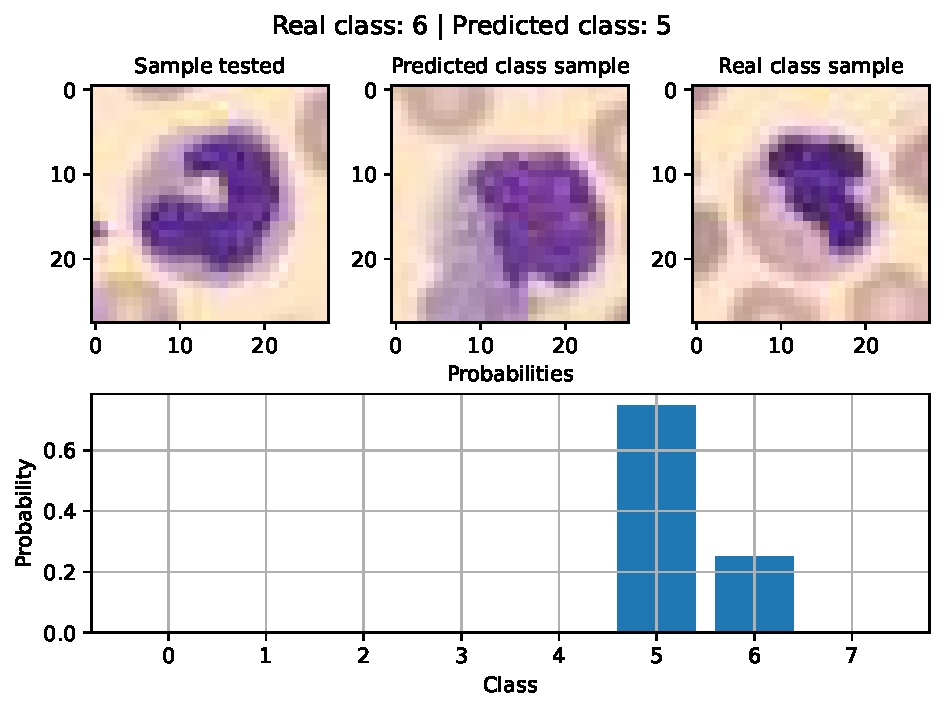
\includegraphics[width=0.75\linewidth]{../../plot/cnn_deep/error_analyser_8}
	\caption{Análise de um caso de erro de classificação.}
	\label{fig:error_analyser_8}
\end{figure}

\begin{figure}[H]
\centering
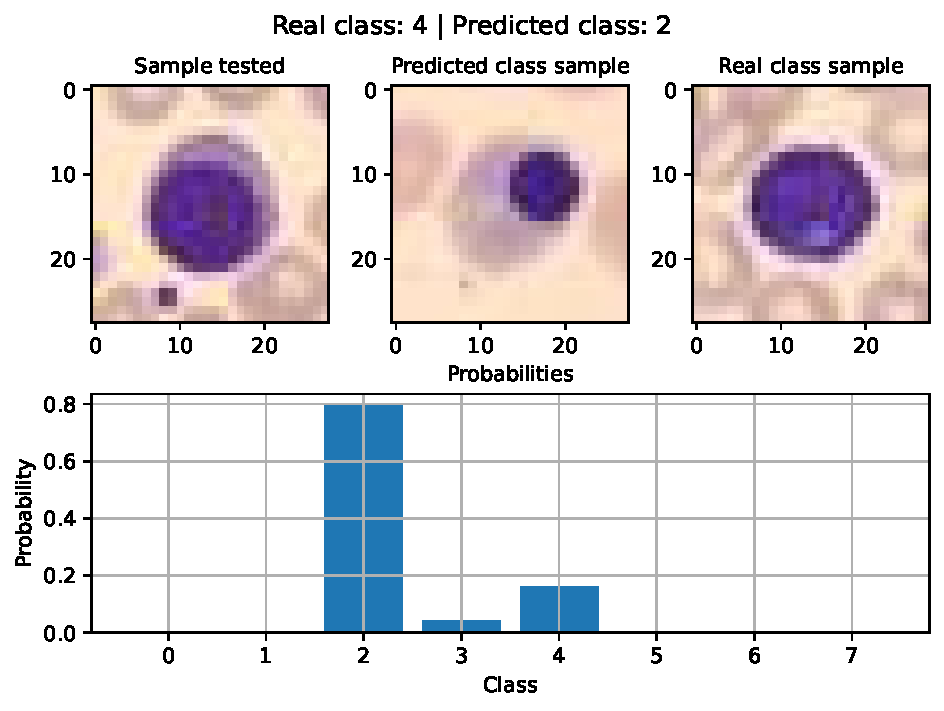
\includegraphics[width=0.75\linewidth]{../../plot/cnn_deep/error_analyser_187}
\caption{Análise de um caso de erro de classificação.}
\label{fig:error_analyser_187}
\end{figure}

\begin{figure}[H]
\centering
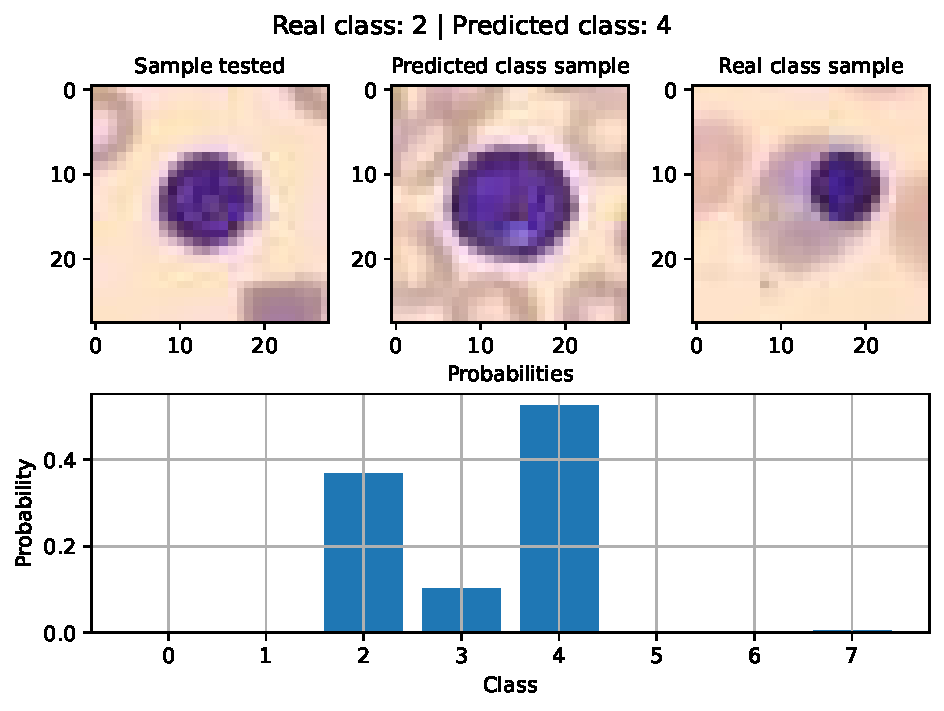
\includegraphics[width=0.75\linewidth]{../../plot/cnn_deep/error_analyser_259}
\caption{Análise de um caso de erro de classificação.}
\label{fig:error_analyser_259}
\end{figure}

\begin{figure}[H]
\centering
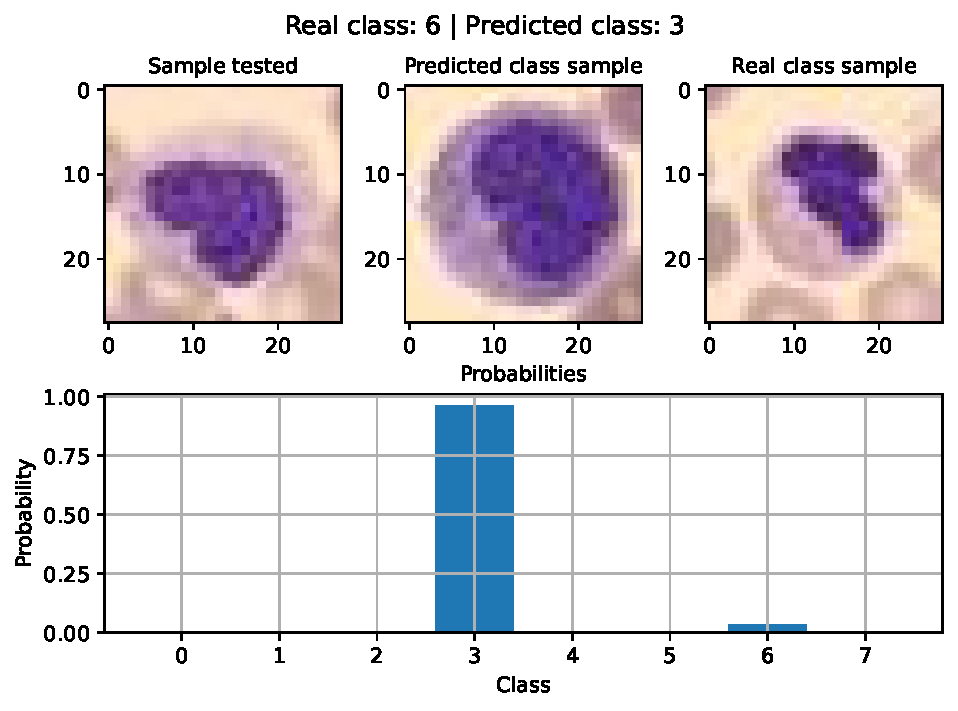
\includegraphics[width=0.75\linewidth]{../../plot/cnn_deep/error_analyser_35}
\caption{Análise de um caso de erro de classificação.}
\label{fig:error_analyser_35_cnn_deep}
\end{figure}

\begin{figure}[H]
\centering
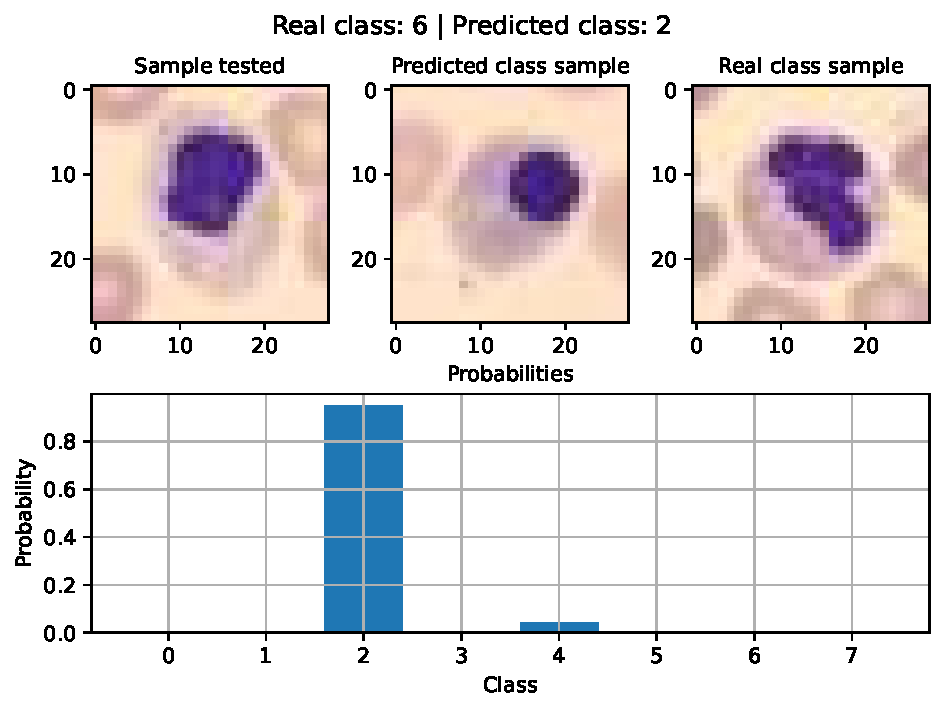
\includegraphics[width=0.75\linewidth]{../../plot/cnn_deep/error_analyser_62}
\caption{Análise de um caso de erro de classificação.}
\label{fig:error_analyser_62_cnn_deep}
\end{figure}

%%%%%%%%%%%%%%%%%%%%%%%%%%%%%%%%%%%%%%%%%%%%%%%%%%%%%%%%%%%%%%%%%%%%%%%%%%%%%%
\clearpage
\section{Conclusão}
